
\documentclass{beamer}

%\usepackage{geometry}
%\geometry{papewidth=20cm,paperheight=20cm}

%\pdfpagewidth 41cm
%\pdfpageheight 29.7cm

\setbeamersize{text margin left=0.1em}  % <- like this
\setbeamersize{text margin right=0.1em} % <- like this

\usepackage{setspace}
\usepackage{varioref}

\newcommand{\q}[1]{{\fontfamily{phv}\selectfont ``}#1{\fontfamily{phv}\selectfont ''}} 


%%??\usepackage{spath3}
%\usepackage{pstricks}

\usepackage{amssymb}
\usepackage{textcomp}
\usepackage{tikz}

\newcommand{\colorbullet}[1]{{\color{#1}\ensuremath{\bullet}}}

%\usetikzlibrary{shapes,snakes}
%%?\usepackage[backslant]{aurical}

%%?\usepackage{hanging}

%\usepackage{DejaVuSerif}

\usepackage{setspace}

\usepackage[outline]{contour}



%{{\color{red!60!yellow}{\textbf{#1}}}}}}}

\usepackage{microtype}
\usepackage{hyphenat}
%%?\usepackage{dashrule}
%\usepackage[usenames,dvipsnames]{xcolor}

\usetikzlibrary{arrows, positioning, shapes}
\usetikzlibrary{backgrounds}


%%?\usepackage{wrapfig}

\usetikzlibrary{arrows, positioning, shapes}

%
%
%\usetheme{Singapore}

%\usetheme{AnnArbor}
%\usecolortheme{spruce}

\usetheme[width=0pt]{BerkeleyAA}
\usecolortheme{spruceaa}

\def\swidth{1cm}
\setbeamersize{sidebar width left=\swidth}
%\addtobeamertemplate{frametitle}{\vspace*{6cm}}{\vspace*{0.3cm}}

\usepackage{mdframed}

\newcommand{\ft}[1]{\vspace*{.25cm}\raisebox{-.45cm}{%
\contour{MSUgreen!50!yellow}{{\protect\Huge{\protect\textbf{#1}}}}}}


%C:/dgch-dev/cpp/testdia/bulletin/reslides/beamerthemeBerkeley.sty
%:/dgch-dev/cpp/testdia/bulletin/reslides/beamerthemeAnnArbor.sty
%C:/dgch-dev/cpp/testdia/bulletin/reslides/beamerthemeAntibes.sty
%C:/dgch-dev/cpp/testdia/bulletin/reslides/beamerthemeBergen.sty

%\usecolortheme{frigatebird}
%\usecolortheme{spruce}
%
%\usetheme{Berlin}
%
%\usecolortheme{spruce}
%\usecolortheme{wolverine}

\setbeamertemplate{blocks}[rounded][shadow=true]
\setbeamertemplate{frametitle}[default][center]
\setbeamertemplate{caption}[numbered]

\beamertemplatenavigationsymbolsempty{}
%\setbeamertemplate{navigationsymbols}{empty}
%\setbeamertemplate{footline}{}
%\setbeamertemplate{footline}[-----]{}
%\setbeamertemplate{headline}{}

\setlength{\paperwidth}{10.in}
\setlength{\paperheight}{7.5in}
\setlength{\textwidth}{9.in}
\setlength{\textheight}{6.5in}

\newcommand{\curlyquote}[1]{{\fontfamily{gar}\selectfont{``}}#1%
{\fontfamily{gar}\selectfont{''}}}

\newcommand{\curlyapos}[1]{{\fontfamily{gar}\selectfont{'}}}

\newcommand{\cfbox}[2]{%
	\colorlet{currentcolor}{.}%
	{\color[rgb]{#1}%
		\fbox{\color{currentcolor}#2}}%
}


%%?\usecolortheme{spruce}

%\setbeamercolor{block title}{red}   
%\setbeamercolor{block title}{red}   

%%\usecolortheme{orchid}
%\usepackage{float}

%\setbeamerfont{itemize/enumerate body}{size=\small}
%\setbeamerfont{normaltext}{size=\}
%\setbeamerfont{block body}{size=\small}
\setbeamerfont{block title}{size=\large}
%\setbeamerfont{block body example}{size=\tiny}

\newcommand{\colortriangle}{{\color[rgb]{0.45, 0.4, 0.28}$\blacktriangleright$}}
	
\newcommand\FourQuad[4]{%
	
	\begin{minipage}[b][.45\textheight][t]{.47\textwidth}#1\end{minipage}\hfill%
	\begin{minipage}[b][.45\textheight][t]{.47\textwidth}#2\end{minipage}\\[0.5em]
	\begin{minipage}[b][.45\textheight][t]{.47\textwidth}#3\end{minipage}\hfill
	\begin{minipage}[b][.45\textheight][t]{.47\textwidth}#4\end{minipage}%
}

\newcommand\ThreeQuad[3]{%
	\hspace{2pt}\begin{minipage}[b][.23\textheight][c]{.99\textwidth}#1\end{minipage}\hfill%
	\begin{minipage}[b][.75\textheight][t]{.55\textwidth}#2\end{minipage}\hfill
	\begin{minipage}[b][.75\textheight][t]{.43\textwidth}#3\end{minipage}%
}

\newcommand\TwoQuad[2]{%
	\begin{minipage}[b][.75\textheight][t]{.55\textwidth}#1\end{minipage}\hfill
	\begin{minipage}[b][.75\textheight][t]{.43\textwidth}#2\end{minipage}%
}

\newcommand\OneQuad[1]{%
	\begin{minipage}[b][.45\textheight][t]{1.01\textwidth}#1\end{minipage}\hfill
	%\begin{minipage}[b][.75\textheight][t]{.43\textwidth}#2\end{minipage}%
}


\newenvironment{quadblock}[1]{\begin{block}{\begin{center}\Large{%
\colorbox[rgb]{0.25,0.1,0.25}{\color{yellow}{\textbf{#1}}}
}\end{center}}%
\begin{minipage}[c]{.97\textwidth}\vspace{1em}
}{
\end{minipage}
\end{block}}


\newenvironment{mpblock}[1]{\begin{block}{\begin{center}\Large{%
\colorbox[rgb]{0.25,0.1,0.25}{\color{yellow}{\textbf{#1}}}
}\end{center}}%
\begin{minipage}[c]{.97\textwidth}\vspace{1em}
\begin{textsf}}{\end{textsf}
\end{minipage}
\end{block}}

\usepackage{aurical}

%%?\usepackage{pbsi}
%\usepackage{oesch}
%\usepackage{LobsterTwo}

%\newcommand{\doubleCenteredFramebox}[1]{%
%\begin{center}%
%\framebox{%
%\begin{minipage}{0.85\textwidth}\begin{center}%
%#1\end{minipage}\end{center}}\end{center}}

%\setlength{\fboxsep}{0.15em}



\newcommand{\doubleCenteredFramebox}[1]{%
\setlength{\fboxsep}{2em}\setlength{\fboxrule}{2pt}
\begin{center}\cfbox{0.1, 0.5, 0.8}{\begin{minipage}{0.85\textwidth}\begin{center}\setlength{\fboxsep}{.25em}#1
	\end{center}\end{minipage}}\end{center}}


\newcommand{\halfPageFramebox}[1]{%
	\setlength{\fboxsep}{2em}\setlength{\fboxrule}{1pt}
	\begin{center}\cfbox{0.1, 0.5, 0.8}{\begin{minipage}{0.5\textwidth}\begin{center}\setlength{\fboxsep}{.25em}#1
				\end{center}\end{minipage}}\end{center}}

\newcommand{\sfitem}[1]{\item \LARGE{\textbf{\textsf{#1}}}}				

\renewcommand*\rmdefault{cmfib}

\newcommand{\scitem}[1]{\item {\Large{{\fontfamily{pag}\selectfont \textbf{#1}}}}}			
\newcommand{\smscitem}[1]{\item {\small{{\fontfamily{pag}\selectfont \textbf{#1}}}}}			


\newcommand{\embitem}[1]{\item \textbf{{\large #1}}}			


\newcommand{\highlightframebox}[1]{\cfbox{1,.5,1}{#1}}

%\begin{minipage}[.45\textheight][t]}{\end{minipage}\end{block}}

\newcommand{\manyasciimacron}{\textasciimacron\textasciimacron\textasciimacron%
\textasciimacron\textasciimacron\textasciimacron\textasciimacron\textasciimacron\textasciimacron%
\textasciimacron\textasciimacron\textasciimacron\textasciimacron\textasciimacron\textasciimacron%
\textasciimacron\textasciimacron\textasciimacron\textasciimacron\textasciimacron\textasciimacron%
}

\newcommand{\manyemdash}{\texttwelveudash\texttwelveudash\texttwelveudash\texttwelveudash\texttwelveudash%
 \texttwelveudash\texttwelveudash\texttwelveudash\texttwelveudash\texttwelveudash\texttwelveudash\texttwelveudash%
 \texttwelveudash\texttwelveudash\texttwelveudash\texttwelveudash\texttwelveudash\texttwelveudash\texttwelveudash%
}

%\usepackage[nodisplayskipstretch]{setspace}

\newenvironment{lightquadblock}[1]{\begin{center}\LARGE{%
			\colorbox[rgb]{.39,0,0.28}{\color[rgb]{1,1,1}{\hspace{-1em}\makebox[\textwidth]{\textbf{#1}}}}
		}\end{center}
		%\begin{framebox}
		\begin{minipage}[c]{.9\textwidth}\vspace{1em}
		}{
	\end{minipage}}
	
\newenvironment{lightquadblockc}[2]{\begin{center}\LARGE{%
			\colorbox[rgb]{#1}{\color[rgb]{1,1,1}{\hspace{-1em}\makebox[\textwidth]{\textbf{#2}}}}
		}\end{center}
		%\begin{framebox}
		\begin{minipage}[c]{.9\textwidth}\vspace{1em}
		}{
	\end{minipage}}

	
	\newenvironment{lightqblock}[1]{\begin{center}\LARGE{%
				\colorbox[rgb]{.90,.90,0.90}{\cfbox{.96,.4,.96}{\color[rgb]{.2,.06,.04}{\hspace{-1em}\makebox[\textwidth]{#1}}}}
			}\end{center}
			%\begin{framebox}
			\begin{minipage}[c]{.99\textwidth}\vspace{1em}
			}{
		\end{minipage}}
		

\newcommand\TwoQuadV[4]{%
	\begin{minipage}[b][.20\textheight][t]{1.04\textwidth}\begin{lightqblock}{#1}#2\end{lightqblock}\end{minipage}
	\begin{center}\begin{minipage}[t][.78\textheight][t]{.9\textwidth}%
		\begin{quadblock}{#3}\begin{minipage}{\textwidth}#4\end{minipage}\end{quadblock}\end{minipage}\end{center}%
}


%\newcommand{\conversationPatterns}{\framebox{%
%Conver\-\\
%sation\\
%Patterns}}

\newcommand{\reParser}{	
\begin{minipage}{32pt}\centering{\begin{scriptsize}\textbf{Relae\\\vspace{-6pt}Parser}\end{scriptsize}} 
\end{minipage}}

\usetikzlibrary{decorations.markings}
\usetikzlibrary{decorations.pathmorphing}

%\newcommand{\q}[1]{``#1"}

\definecolor{quadgrey}{rgb}{.9,.9.,.89}
\colorlet{snakegrey}{black!80!white}
\colorlet{blbl}{blue!20!black}

\definecolor{lqboutercolor}{rgb}{.92,.91,0}
\definecolor{lqbinnercolor}{rgb}{.98,.98,.98}

\definecolor{blGreen}{rgb}{.2,.7,.3}
\definecolor{darkRed}{rgb}{.2,.0,.1}

\definecolor{postLinkColor}{rgb}{.5,.5,.1}

\definecolor{fcBoxColor}{rgb}{.8,.6,.3}

\definecolor{BlueGreen}{rgb}{.1,.6,.4}

\colorlet{ry}{red!80!yellow}
\colorlet{rblue}{red!70!blue}
\colorlet{rb}{rblue!40!black}
\colorlet{bg}{blGreen!40!black}

\newcommand{\hc}[1]{{\Huge %
{\contour{ry}{\protect\contour{rb}{{\protect\color{blGreen!40!black}{\protect\textbf{#1}}}}}}}}

\colorlet{yy}{yellow!80!blue}
\colorlet{yo}{yellow!80!orange}
\colorlet{yw}{yellow!20!white}



%\usepackage{microtype}

%\usepackage{mathtools}

\newcommand{\yhc}[1]{{ %
{\contourlength{1.2pt}
{{\protect\contour{yw!50}{\protect\contour{yo!50}{{\protect\color{yy}{\protect\textbf{%
{\protect\Huge{\protect\textls[240]{#1}}}}}}}}}}}}}


\newcommand{\cframedbox}[1]{\begin{mdframed}
[linecolor=rb!85!red,linewidth=0.4mm]#1\end{mdframed}}

\newcommand{\cframedboxpanda}[1]{\begin{mdframed}
		[linecolor=yellow!70!blue,linewidth=0.8mm]#1\end{mdframed}}

\newcommand{\cframedboxblue}[1]{\begin{mdframed}
		[linecolor=blue!70!black,linewidth=0.8mm]#1\end{mdframed}}


\newcommand{\cframedboxx}[3]{\begin{mdframed}
		[linecolor=rb!85!red,linewidth=#2]\hspace{#1}#3\end{mdframed}}

\newcommand{\cframedboxyellow}[1]{\begin{mdframed}
[linecolor=rb!45!yellow,linewidth=0.4mm]#1\end{mdframed}}

\newenvironment{postfragment}{\begin{minipage}{5.4cm}\begin{small}}
{\end{small}\end{minipage}}

\newenvironment{postComment}{\begin{minipage}{8cm}\begin{small}}
{\end{small}\end{minipage}}

\newenvironment{postLongComment}{\begin{minipage}{9cm}\begin{small}}
		{\end{small}\end{minipage}}


\newenvironment{tightcenter}{%
	\setlength\topsep{0pt}
	\setlength\parskip{0pt}
	\begin{center}
	}{%
\end{center}
}

\newcommand{\tightcenterline}[1]{\begin{tightcenter}#1\end{tightcenter}}



\definecolor{postBkgColor}{rgb}{.95,.85,.95}
\definecolor{postCommentBkgColor}{rgb}{.85,.85,.95}

\definecolor{grammarArrowColor}{rgb}{.85,.85,.45}

\tikzstyle{postStyle}=[draw=yellow!120,rounded corners,fill=postBkgColor,thin,inner sep=.2cm]
\tikzstyle{postCommentStyle}=[draw=postCommentBkgColor,double,fill=postCommentBkgColor,thick,inner sep=.2cm]

\tikzstyle{sdComponent}=[double,rounded corners,draw=brown!120,fill=blue!50,thin,inner sep=.2cm]
\tikzstyle{cnvComponent}=[double,shape=diamond,rounded corners,draw=brown!120,fill=blue!50,thin,inner sep=0cm]

\tikzstyle{baseStyle}=[fill=purple!50,draw=cyan!20,ultra thick,double,shape=diamond,inner sep=.15cm]
\tikzstyle{componentStyle}=[fill=red!50,draw,shape=ellipse,inner sep=.15cm]

\tikzstyle{componentExtendedStyle}=[fill={rgb:red,10;green,10;blue,2},draw,shape=rectangle,inner sep=.15cm]

\newcommand{\emphcolor}{%
	\colorlet{currentcolor}{.}%
	\color[rgb]{.4,.4,.4}}

\newcommand{\ncolor}{%
	\color{currentcolor}}


\definecolor{slidePartHeadColor}{rgb}{0,.2,.1}

\newcommand{\slidePartHead}[1]{{\fontfamily{pnc}\selectfont\color{slidePartHeadColor}\LARGE#1}}

\newcommand{\slidePartHeadCenter}[1]{\slidePartHead{\begin{minipage}{\textwidth}\begin{center}#1\end{center}\end{minipage}}}

\newcommand{\componentLabel}[1]{\begin{minipage}{3.5cm}\begin{center}#1\end{center}\end{minipage}}
\newcommand{\baseComponentLabel}[1]{\begin{minipage}{2cm}\textbf{\begin{center}#1\end{center}}\end{minipage}}

\newcommand{\componentExtendedLabel}[1]{\begin{minipage}{10cm}\begin{center}\textbf{#1}\end{center}\end{minipage}}

\newcommand{\cstd}[1]{\textbf{{\color[rgb]{.4,.4,.1}#1}}}

\usepackage{setspace}

%\fontfamily{pag}\selectfont \textbf{
\newcommand{\raiseBoxL}[1]{\makebox{\raisebox{.1em}{{\fontfamily{put}\fontseries{sb}\selectfont #1}\hspace{1.2em}}}}
%	\begin{textsf}{\small}{}\end{textsf}\end{minipage}}

\newcommand{\doubleFrame}[1]{\doubleFrameX{.98\textwidth}{#1}}

\newcommand{\doubleFrameX}[2]{\doubleFrameXX{2pt}{#1}{#2}}

\newcommand{\doubleFrameXX}[3]{%
	\fcolorbox{fcBoxColor!90!cyan}{gray!50}{
		%{\begin{center}
		\begin{minipage}{.985\textwidth}
			%\begin{center}	
			\hspace{#1}\vspace*{1pt}		
			\fcolorbox{fcBoxColor!50!cyan}{white}{%
				\begin{minipage}{#2}%
					\begin{center}\begin{minipage}{.97\textwidth}				
							\begin{spacing}{1.8}\vspace{.5em}{\textbf{\Large #3}\vspace{-20pt}}\end{spacing}%
						\end{minipage}\end{center}
					\end{minipage}}
					%\end{center}
				\end{minipage}}
				%\end{center}}
			}%
			

\newcommand{\doubleFrameXspec}[3]{%
	\fcolorbox{fcBoxColor!90!cyan}{gray!50}{
		%{\begin{center}
		\begin{minipage}{\textwidth}
			%\begin{center}	
			\hspace{#1}\vspace*{1pt}		
			\fcolorbox{fcBoxColor!50!cyan}{white}{%
				\begin{minipage}{#2}%
					\begin{center}\begin{minipage}{.99\textwidth}				
							\begin{spacing}{1.8}\vspace{.5em}{\textbf{\Large #3}\vspace{-20pt}}\end{spacing}%
						\end{minipage}\end{center}
					\end{minipage}}
					%\end{center}
				\end{minipage}}
				%\end{center}}
			}%
			



\newcommand{\doubleFrameY}[6]{%
	\fcolorbox{fcBoxColor!90!black}{gray!50}{
		\setlength{\fboxsep}{#5}%{\begin{center}
		\begin{minipage}{#1}
			%\begin{center}	
			\hspace{#2}\vspace*{1pt}		
			\fcolorbox{fcBoxColor!50!black}{white}{%
\begin{minipage}{#3}%
					\begin{center}\begin{minipage}{#4}				
							\begin{spacing}{1.8}\vspace{.5em}{\textbf{\Large #6}\vspace{-20pt}}\end{spacing}%
						\end{minipage}\end{center}
					\end{minipage}}
					%\end{center}
				\end{minipage}}
				%\end{center}}
			}%
			
			


\usepackage{aurical}
\usepackage[T1]{fontenc}
\usepackage{libris}
\usepackage{relsize}

\newcommand{\VersatileUX}{{\color{red!85!black}\Fontauri Versatile}%
{{\fontfamily{qhv}\selectfont\smaller UX}}}


\newcommand{\doubleFrameTwo}[2]{%
\begin{center}
\begin{minipage}{\textwidth}	
\fcolorbox{fcBoxColor!50}{gray!50}{
%	\begin{center}
\begin{minipage}{\textwidth}
	\begin{center}
			%\hspace{4pt}\vspace*{2pt}		
			\fcolorbox{fcBoxColor!90}{white}{%
				\begin{minipage}{.95\textwidth}%
\begin{center}\begin{minipage}{.91\textwidth}#1\end{minipage}\end{center}%
				\end{minipage}}\vspace*{.5em}\\
%\vspace*{2pt}
%\hspace{4pt}				
\fcolorbox{fcBoxColor!90}{white}{
		\begin{minipage}{.94\textwidth}
\begin{center}\begin{minipage}{.91\textwidth}#2\end{minipage}\end{center}%
		\end{minipage}}
\end{center}		
\end{minipage}
%
}\par 
\end{minipage}
\end{center}		
}

\newcommand{\itup}[1]{\raisebox{2pt}{{\normalsize(#1)}}}

\newcommand{\FER}{{\color[rgb]{0.1,0.25,0.6}{FER}}}
\newcommand{\BER}{{\color[rgb]{0.1,0.25,0.6}{BER}}}
\newcommand{\IR}{{\color[rgb]{0.1,0.25,0.6}{IR}}}

\newcommand{\FrontEnd}{{\color[rgb]{0.1,0.25,0.6}{Front-End}}}
\newcommand{\BackEnd}{{\color[rgb]{0.1,0.25,0.6}{Back-End}}}
\newcommand{\Intermediate}{{\color[rgb]{0.1,0.25,0.6}{Intermediate}}}

%\newcommand{\doubleFrameTwo}[2]{%
%\fcolorbox{fcBoxColor}{gray!50}{
%\begin{minipage}{.98\textwidth}
%\hspace{4pt}\vspace*{2pt}	
%\fcolorbox{fcBoxColor}{white}{%
%\begin{minipage}{.95\textwidth}#1
%\end{minipage}}#1
%\fcolorbox{fcBoxColor}{white}{%
%\begin{minipage}{.95\textwidth}#2%
%\end{minipage}}
%}


%\newenvironment{doubleFrame}{%
%\fcolorbox{fcBoxColor}{gray!50}{\begin{minipage}{\textwidth}}
%{\end{minipage}}}

%\newenvironment{doubleFrame}{% \fcolorbox{fcBoxColor}{gray!50}{%
%\fbox{\begin{minipage}{\textwidth}%
%}
%{\end{minipage}}}
%}}
\usetikzlibrary{shadows}
\definecolor{logoRed}{rgb}{.3,0,0}
\definecolor{logoPeach}{RGB}{255, 159, 102}
\definecolor{logoCyan}{RGB}{66, 206, 244}
\definecolor{logoBlue}{RGB}{4, 2, 25}

\usepackage{changepage}

\newcommand{\nodeincludegraphicsLOCTRV}[7]{
\node[anchor=south west,inner sep=0,thick,
drop shadow={top color=logoBlue!50!logoCyan,
              bottom color=logoRed!50!logoCyan,
              shadow xshift=-1pt,
              shadow yshift=-3pt,
              rounded corners}] (image) at (#1){%
\fcolorbox{logoRed}{logoPeach!40!logoRed}{\includegraphics[scale=#2,trim={#5 #4 #3 #6},clip]{#7}}};}

%\newcommand{\doubleFrame}[1]
\newcommand{\nodeincludegraphics}[2][0.8\textwidth]{
\node[anchor=south west,inner sep=0] (image) at (0,0){%
\includegraphics[width=#1]{#2}};}

\newcommand{\nodeincludegraphicsR}[2][1]{
\node[anchor=south west,inner sep=0] (image) at (0,0){%
\includegraphics[scale=#1]{#2}};}

\newcommand{\nodeincludegraphicsAS}[1]{
\node[anchor=south west,inner sep=0] (image) at (0,0){%
\includegraphics{#1}};}

%\newcommand{\nodeincludegraphicsLOC}[3]{
%\node[anchor=south west,inner sep=0] (image) at (#1){%
%\includegraphics[scale=1]{#3}};}

\newcommand{\nodeincludegraphicsLOC}[3]{
\node[anchor=south west,inner sep=0] (image) at (#1){%
\includegraphics[scale=#2]{#3}};}

\newcommand{\nodeincludegraphicsTRRSqqq}[6]{
\node[anchor=south west,inner sep=0] (image) at (0,0){%
\includegraphics[scale=#1,trim={#2 #3 #4 #5},clip]{#6}};}

\newcommand{\nodeincludegraphicsTR}[3]{
\node[anchor=south west,inner sep=0] (image) at (0,0){%
\includegraphics[trim={0 #2 #1 0},clip]{#3}};}

\newcommand{\nodeincludegraphicsTRR}[5]{
	\node[anchor=south west,inner sep=0] (image) at (0,0){%
		\includegraphics[trim={#3 #2 #1 #4},clip]{#5}};}

\newcommand{\nodeincludegraphicsTRRS}[6]{
\node[anchor=south west,inner sep=0,scale=#1] (image) at (0,0){%
\includegraphics[trim={#4 #3 #2 #5},clip]{#6}};}


\newcommand{\ann}[9]{%
	\path [draw=#1,draw opacity=#2,line width=#3, fill=#4, fill opacity = #5, even odd rule] %
	(#6) ellipse(#7 and #8) ellipse(#7*#9 and #8*#9);}

\newcommand{\polyann}[9]{%
\path [draw=#1,draw opacity=#2,line width=#3, fill=#4, fill opacity = #5, even odd rule] %
	node [minimum size=#8,regular polygon,regular polygon sides=#7] at (#6) {}
	node [minimum size=#9,regular polygon,regular polygon sides=#7] at (#6) {};}
	

%\newcommand{\polyann}[9]{%
%	\path [draw=#1,draw opacity=#2,line width=#3, fill=#4, fill opacity = #5, even odd rule] %
%	path minimum size=2cm,regular polygon,regular polygon sides=6(#7 and #8) ellipse(#7*#9 and %#8*#9);}


\makeatletter
\newcommand*\getX[1]{\expandafter\getX@i#1\@nil}
\newcommand*\getY[1]{\expandafter\getY@i#1\@nil}
\def\getX@i#1,#2\@nil{#1}
\def\getY@i#1,#2\@nil{#2}
\makeatother

\newcommand{\rectann}[9]{%
	\path [draw=#1,draw opacity=#2,line width=#3, fill=#4, fill opacity = #5, even odd rule] %
	(#6) rectangle(\getX{#6}+#7,\getY{#6}+#8)
	({\getX{#6}+((#7-(#7*#9))/2)},{\getY{#6}+((#8-(#8*#9))/2)}) rectangle %
	({\getX{#6}+((#7-(#7*#9))/2)+#7*#9},{\getY{#6}+((#8-(#8*#9))/2)+#8*#9});}

\newcommand{\rectanneatdbl}[9]{%
	\path [draw=#1,draw opacity=#2,line width=#3, fill=#4, fill opacity = #5, even odd rule] %
	(#6) rectangle(\getX{#6}+#7,\getY{#6}+#8)
	({\getX{#6}+\getX{#9}},{\getY{#6}+\getY{#9}}) rectangle %
	({\getX{#6}+#7-\getX{#9}},{\getY{#6}+#8-\getY{#9}})
	;}

\newcommand{\rectanneat}[9]{%
	\path [draw=#1,draw opacity=#2,line width=#3, fill=#4, fill opacity = #5, even odd rule] %
	(#6) rectangle(\getX{#6}+#7,\getY{#6}+#8)
	({\getX{#6}+(#7/abs(#7))*#9},{\getY{#6}+(#8/abs(#8))*#9})
	rectangle({\getX{#6}+#7-(#7/abs(#7))*#9},{\getY{#6}+#8-(#8/abs(#8))*#9});}

\newcommand{\colorarr}[8]{
	\draw [#1, draw=#2,draw opacity=#3,
	fill=#4,fill opacity=#5,line width=#6] (#7) to (#8);
}

\colorlet{brred}{brown!53!red}
\colorlet{grred}{grammarArrowColor!40!red!60}

\definecolor{elColor}{rgb}{.2,.1,0}
\definecolor{flColor}{rgb}{0.7,0.3,0.3}

\definecolor{logoOrange}{RGB}{108, 18, 30}
\definecolor{logoGreen}{RGB}{85, 153, 89}
\definecolor{logoPurple}{RGB}{200, 208, 30}

\definecolor{logoBlue}{RGB}{4, 2, 25}
\definecolor{logoPeach}{RGB}{255, 159, 102}
\definecolor{logoCyan}{RGB}{66, 206, 244}
\definecolor{logoRed}{rgb}{.3,0,0}



\newcommand*{\MyDiamond}{%
	\begin{tikzpicture}{baseline}	
	\node [draw, shape=diamond, %shape border rotate=100,
	line width=.2mm, left color=flColor, right color=darkRed, draw=logoPurple, aspect=1,
	draw opacity=0.6, fill opacity=0.8, xscale=0.5, yscale=0.5,
	minimum width=1mm, 
	] 
	at (2, 0) {};\end{tikzpicture}}

%\usetikzlibrary{shapes.geometric}

\newcommand*{\MyOctagon}{%
	\begin{tikzpicture}{baseline}	
	\node [draw, regular polygon, regular polygon sides=8, %shape border rotate=100,
	line width=.2mm, left color=blue!60!cyan, right color=yellow!30!cyan, draw=blue!50!red, aspect=.7,
	draw opacity=.8, fill opacity=0.8, xscale=0.7, yscale=0.7,
	minimum width=1mm, 
	] 
	at (0, 0) {};\end{tikzpicture}}

\newcommand*{\MyOct}{\hspace{14pt}\raisebox{1pt}{\MyOctagon}\hspace{13pt}}
	
%\usetikzlibrary{fadings}

\newcommand*{\MySquare}{%
	\begin{tikzpicture}{baseline}
	\node [draw, %shape border rotate=100,
	line width=1pt, left color=blue!60!cyan, right color=yellow!30!cyan, draw=cyan!30!blue, aspect=1,
	%path fading=south,
	draw opacity=0.8, fill opacity=1, 
	xscale=0.75, yscale=0.75,
	minimum width=.4mm, shading angle=60
	] 
	at (0, 0) {};

  \draw[draw=red!70!orange,draw opacity=0.5,] (-.14,-.14) -- (.14,-.14) -- (.14,.14);
  
	
%			\node [draw, 
%			line width=1pt, draw=red,
%			draw opacity=0.3, fill opacity=0, 
%			xscale=0.8, yscale=0.8,
%			minimum width=.4mm
%			] 
%			at (0, 0) {};	
			
	\end{tikzpicture}}

\newcommand{\sqitem}{\item[\raisebox{2pt}{\MySquare}]}
\newcommand{\dmitem}{\item[\raisebox{2pt}{\MyDiamond}]}

\newcommand{\nodeincludegraphicsLOCTR}[7]{
\node[anchor=south west,inner sep=0,thick,
drop shadow={top color=logoBlue!50!logoCyan,
              bottom color=logoRed!50!logoCyan,
              shadow xshift=-1pt,
              shadow yshift=-3pt,
              rounded corners}] (image) at (#1){%
\fcolorbox{logoRed}{logoPeach!40!logoRed}{\includegraphics[scale=#2,trim={#5 #4 #3 #6},clip]{#7}}};}


\newcommand{\lsep}{\hspace{7pt}}
\newcommand{\llsep}{\hspace{14pt}}

\usepackage[official]{eurosym}

\usetikzlibrary{shadings}
\usepackage{pgf-pie}


\newcommand{\AtR}{A{\smaller{3}}R}

%\usepackage[official]{eurosym}

\newcommand{\thrule}{\vspace{.5em}{%
\color[RGB]{200,47,100}{\hrule}\vspace{3pt}
\color[RGB]{164,67,19}{\hrule}}\vspace{.9em}}

\newcommand{\thrulex}{\vspace{-1.5em}{%
\color[RGB]{14,67,19}{\hrule  height 8pt}\vspace{-2pt}
\color[RGB]{10,47,100}{\hrule height 8pt}}\vspace{2.3em}}

\usepackage{pdfpages}


\colorlet{lplr}{logoPeach!40!logoRed}

%%%%%%%%%%%%%%%%%%%%%%%%%%%%%%%%%%%%%%%%%%%%%%%%%%%%%%%%%%%%%%%%%%%%%%
%\annotatedFigureBoxCustom{bottom-left}{top-right}{label}{label-position}{box-color}{label-color}{border-color}{text-color}
\newcommand*\annotatedFigureBoxCustom[8]{\draw[#5,thick,rounded corners] (#1) rectangle (#2);\node at (#4) [fill=#6,thick,shape=circle,draw=#7,inner sep=2pt,font=\sffamily,text=#8] {\textbf{#3}};}
%\annotatedFigureBox{bottom-left}{top-right}{label}{label-position}
\newcommand*\annotatedFigureBox[4]{\annotatedFigureBoxCustom{#1}{#2}{#3}{#4}{lplr}{grred!30!black}{brred}{brred!20}}
\newcommand*\annotatedFigureText[4]{\node[draw=none, anchor=south west, text=#2, inner sep=0, text width=#3\linewidth,font=\sffamily] at (#1){#4};}
\newenvironment {annotatedFigure}[3]{\vspace*{#2}\hspace*{#1}\centering\begin{tikzpicture}
    \node[anchor=south west,inner sep=0] (image) at (0,0) {#3};\begin{scope}[x={(image.south east)},y={(image.north west)}]}{\end{scope}\end{tikzpicture}}

%%%%%%%%%%%%%%%%%%%%%%%%%%%%%%%%%%%%%%%%%%%%%%%%%%%%%%%%%%%%%%%%%%%%%%

\definecolor{logoYellow}{RGB}{255, 249, 232}

\newcommand{\sovn}[1]{\color{yellow!20!logoYellow}{{\textbf{#1}}}}

\newcommand{\mybox}[1]{\raisebox{1pt}{{\small\colorbox{grred!30!black}{\parbox{2mm}{\sovn{#1}}}}}}

\newcommand{\circled}[1]{{\mybox{#1}}}



\usepackage{eso-pic}

\newcommand{\atspt}{%
	\AddToShipoutPicture*{%
		\raisebox{16.5cm}{\hspace{25.5cm}\parbox{6cm}{%
				
\includegraphics[width=6cm]{e-logo.png}
			}}}}


\newcommand{\atsp}{%
\AddToShipoutPicture*{%
\raisebox{9.5cm}{\hspace{25.5cm}\parbox{6cm}{%

\includegraphics[width=6cm]{e-logo.png}\\

\vspace*{6cm}

\begin{center}
Linguistic Technology Systems\\

\includegraphics[width=4cm]{logo.png}
\end{center}
	
}}}}

%\raisebox{4cm}{\hspace{26cm}
\includegraphics[width=8cm]{logo.png}}


\setbeamercolor{background canvas}{bg=}

\makeatletter
\define@key{Gin}{resolution}{\pdfimageresolution=#1\relax}
\makeatother

\newcommand{\annfont}{\fontsize{13}{15}\selectfont}

\begin{document}
	
	\pdfpagewidth 32cm
%	\pdfpageheight 30cm
	
\part{ScreenShots}
%\section{Group_1-1-intro}
\atsp
\begin{frame}{\parbox{20cm}{\centering\ft{Dataset Creator}\\ 
%\ft{\fontsize{23}{22}\selectfont Integrated with Cloud Back-Ends}\\ 
\ft{\LARGE{(\curlyquote{dsC})}}}}
\section{Intro}
\vspace{-2em}

%\colorbox{cyan}{
%\begin{minipage}{.43\textwidth}
%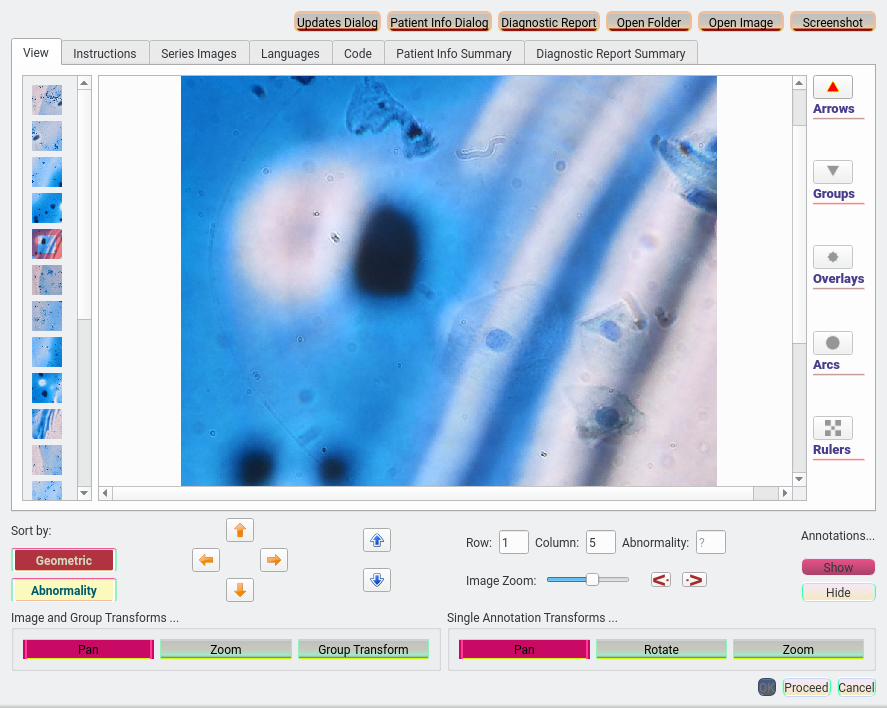
\includegraphics[scale=.5]{slide1pic1.png}
%\end{minipage}\begin{minipage}{.5\textwidth}
%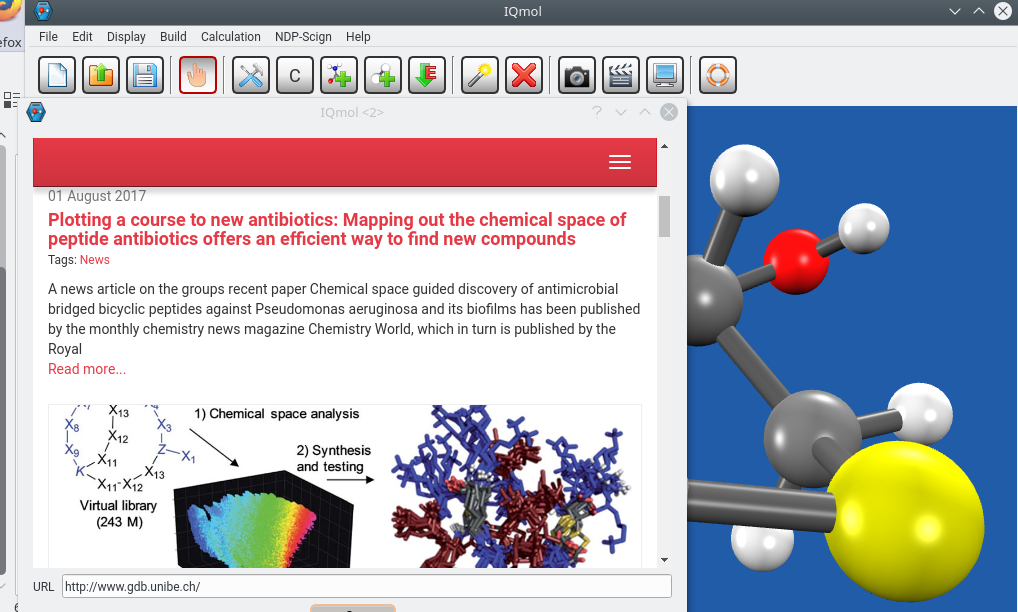
\includegraphics[scale=.5]{slide1pic1a.png}
%\end{minipage} }

\definecolor{pd}{RGB}{200,60,30}

%\begin{adjustwidth*}{-2em}{} 
\hspace*{10pt}\begin{tikzpicture}

%\node [fill=white] at (20,0) {PITCH DECK};


\nodeincludegraphicsLOCTR{13.6,3.7}{0.35}{4cm}{0cm}{1cm}{0cm}{after/slide1pic1a.png}

\nodeincludegraphicsLOCTR{17,0.1}{0.3}{0cm}{0cm}{0cm}{0cm}{after/Pub-4.png}


\nodeincludegraphicsLOCTR{0,0}{0.64}{1.2cm}{4cm}{1cm}{1cm}{after/slide1pic1.png}

\end{tikzpicture}
%\end{adjustwidth*}



\vspace{.5em}
		
%\hspace{2m}
\colorbox{white}
{%
\setlength{\fboxsep}{0pt}{\parbox{\textwidth}{%			
\begin{center}
\colorbox[RGB]{200,60,30}	
{\setlength{\fboxsep}{8pt}				
\hspace{3pt}\colorbox{white}{\setlength{\fboxsep}{0pt}
%\framebox{
\LARGE\begin{minipage}{.85\textwidth}
\vspace{4pt}\centering
Linguistic Technology Systems (LTS) \\
Amy Neustein, Ph.D., Founder and CEO \\
amy.neustein@verizon.net \\
(917) 817-2184 
\end{minipage}
%}
}
\hspace{1pt}
}
\end{center}
}}
}
\end{frame}

\atsp
\begin{frame}{\ft{Group 1: Features of Dataset Applications}}
	
%{\begin{minipage}{35cm}\ft{Group 1: Features of Dataset Applications}\hspace{7.4cm}\colorbox{purple!40!black}{\hspace{10cm}}\end{minipage}}
\vspace{-13em}
\OneQuad
{
\begin{quadblock}{User Interface Features Typical of Dataset Applications}
\hspace{1cm}{\parbox{19cm}{\LARGE
\fontseries{b}\selectfont
{
The code for each dsC data set includes a 
customized \curlyquote{Dataset Application} which displays 
individual samples and groups of samples via 
2D, 3D, and native-compiled GUI controls.  
Each Dataset Application can thereby make use of 
advanced visual and interactive features that 
are uniquely possible when using 
customized, native-compiled GUI classes.  
The following screenshots will 
show several examples of these features, such as:
\vspace{1em} 


\begin{description}
\item[Specialized Top-Level Controls] Tree Widgets, Stacked Widgets, and Graphics Scenes.
\item[Context Menus] Systematically organizes functionality premised on UI layouts.
\item[Multi-Window Displays] Divides application functionality into  multiple top-level windows and/or dialog boxes.
\end{description}
}
}}
\end{quadblock}
}
\end{frame}

\atsptt
    \begin{frame}{\ft{Initial Application Window}}
\pdfpageheight 30cm
\section{Group 1: Initial Application Window}
\vspace{19pt}
        \begin{annotatedFigure}{10pt}{0pt}
            {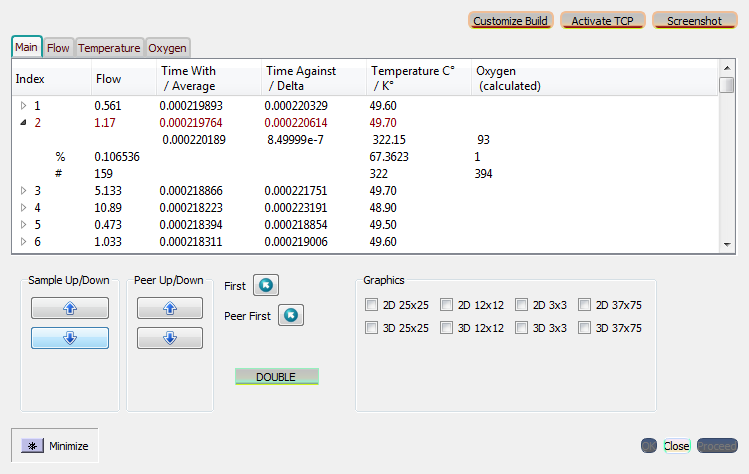
\includegraphics[scale=1.5]{texs/expand.png}}
            
  \node [
  line width=1mm, fill opacity=0.9,
  draw = logoCyan!50!logoBlue,
  bottom color=logoCyan!40,text=black,
  top color=logoCyan!10,
  rounded corners=6pt,
  text width=9.2cm, inner sep=14pt]
   at (0.74,0.465){\annfont\textbf{Using a ``tree widget" (a two-layer spreadsheet), 
  instead of a conventional spreadsheet, allows the Dataset Application to 
  distinguish primary values (those measured directly by physical devices 
  and experimental equipment) from intermediate values calculated via algorithms.}};
              
            \annotatedFigureBox{0.01,0.6}{0.75,0.77}{1}{0.75,0.6}
            
  \node [text width=7.5cm, inner sep=14pt,align=justify,
    line width=1mm, fill opacity=0.9,
    draw = logoCyan!50!logoBlue,
    top color=logoCyan!40,text=black,
    bottom color=logoCyan!10,
    rounded corners=6pt,
    text width=9cm, inner sep=14pt]
   at (0.23,0.482){\annfont\textbf{In addition, nested rows can 
   display supplemental information, such as data values' 
   rank (\circled{3}) and percentage (\circled{2}) 
   (on the scale of the least to greatest 
   value) relative to all other values for each statistical parameter.}};
              
            \annotatedFigureBox{0.015,0.65}{0.1,0.69}{2}{0.1,0.69}
            \annotatedFigureBox{0.015,0.62}{0.1,0.648}{3}{0.1,0.625}                        
            
            
            
            %bl
      %      \annotatedFigureBox{0.222,0.284}{0.3743,0.4934}{B}{0.3743,0.4934}%tr
      %      \annotatedFigureBox{0.555,0.784}{0.6815,0.874}{C}{0.555,0.784}%bl
      %      \annotatedFigureBox{0.557,0.322}{0.8985,0.5269}{D}{0.8985,0.5269}%tr
  

        \end{annotatedFigure}

   %     \caption{Expanded Sample (A)}
    %    \label{fig:teaser}

    \end{frame}



\atsptt
    \begin{frame}{\ft{Interacting with the Main Window}}
\section{Group 1: Interacting with the Main Window}

        \begin{annotatedFigure}{18pt}{0pt}
            {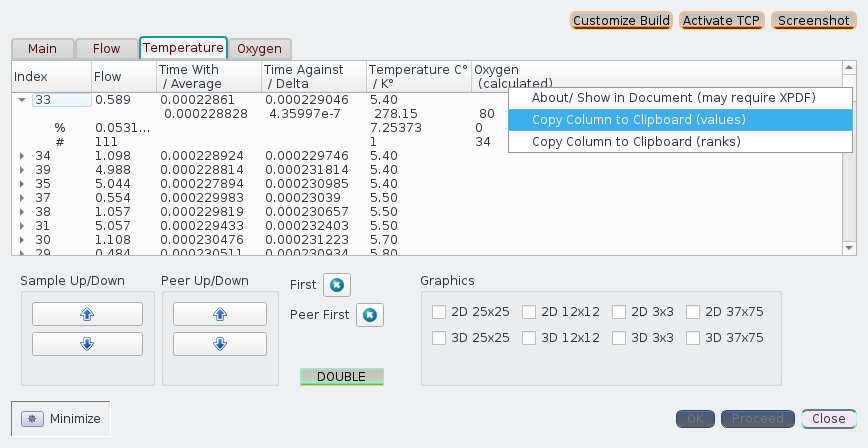
\includegraphics[scale=1.25]{texs/copy.png}}
            
  \node [text width=10cm,inner sep=14pt,align=justify,fill=logoCyan!20, draw=logoBlue, 
  draw opacity=0.5,line width=1mm, fill opacity=0.9]
   at (0.76,0.47){\annfont\textbf{Despite being implemented as a tree widget 
   instead of a two-dimensional spreadsheet, the primary 
   window for this Dataset Application has many speadsheet-like 
   features, such as copying columns of data 
   (\circled{1}) and sorting columns by switching 
   notebook tabs  (\circled{2}); each notebook page shows the data sorted 
   on a specific parameter.}};


      \annotatedFigureBox{0.93,0.67}{0.93,0.71}{1}{0.93,0.663}%
      \annotatedFigureBox{0.01,0.86}{0.34,0.935}{2}{0.17,0.85}% 
            
  \node [text width=11cm,inner sep=14pt,align=justify,fill=logoCyan!20, draw=logoBlue, 
  draw opacity=0.5,line width=1mm, fill opacity=0.9]
   at (0.59,0.2){\annfont\textbf{Two different sets of navigation buttons 
   enable the user to scroll through samples according to 
   the currently selected sort \mbox{parameter} (\circled{3}), 
   or according to the primary index (\circled{4}).}};

   \annotatedFigureBox{0.18,0.18}{0.33,0.41}{3}{0.33,0.41}%
   \annotatedFigureBox{0.02,0.18}{0.17,0.41}{4}{0.02,0.41}%    
      %      \annotatedFigureBox{0.222,0.284}{0.3743,0.4934}{B}{0.3743,0.4934}%tr
      %      \annotatedFigureBox{0.555,0.784}{0.6815,0.874}{C}{0.555,0.784}%bl
      %      \annotatedFigureBox{0.557,0.322}{0.8985,0.5269}{D}{0.8985,0.5269}%tr
  
        \end{annotatedFigure}

   %     \caption{Expanded Sample (A)}
    %    \label{fig:teaser}

    \end{frame}



\begin{frame}{\ft{Coordinated Data Visualization}}
\section{Group 1: Coordinated Data Visualization}

	\pdfpageheight 30cm
	
\begin{annotatedFigure}{2mm}{-1mm}{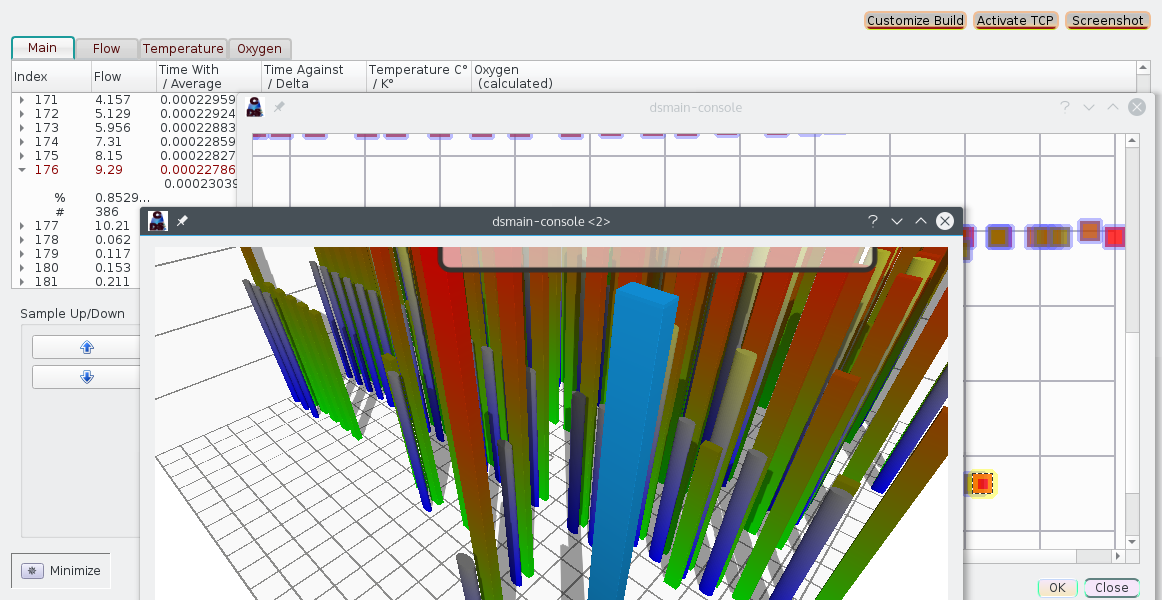
\includegraphics[scale=1]{texs/coord.png}}
  \node [anchor=west,inner sep=14, text width=8.7cm,
  line width=1mm, fill opacity=0.9,
  draw = blue!20!black,
  top color=white,text=black,
  bottom color=blue!40,
  rounded corners=6pt
  %blur shadow={shadow blur steps=2}
  ]
  at (0.67,0.72){\annfont\textbf{Dataset Applications can use 2- and 3D 
  		visualization as well as textual/tabular displays, employing Reactive 
  		Programming techniques to coordinate multiple visible windows.  For example, 
  		visual cues direct attention to selected samples represented via 
  		expanded rows (\circled{1}), color-highlighted 2D regions (\circled{2}), 
  		and color-highlighted 3D bars (\circled{3}).  The main, 2D, 
  		and 3D windows are functionally linked so that the same sample is 
  		highlighted/expanded in each display window.}};
  
              \annotatedFigureBox{0.02,0.63}{0.057,0.74}{1}{0.057,0.74}%
              \annotatedFigureBox{0.825,0.16}{0.86,0.23}{2}{0.856,0.24}%            
              \annotatedFigureBox{0.55,0.42}{0.55,0.48}{3}{0.55,0.48}     
              
\end{annotatedFigure}	
%\end{figure}
\end{frame}



\begin{figure}

\caption{Data Microcitations via Tabular Columns}
\label{fig:oxy}

\begin{tikzpicture}

\node[inner sep=0pt] (x1) at (0,0)
    {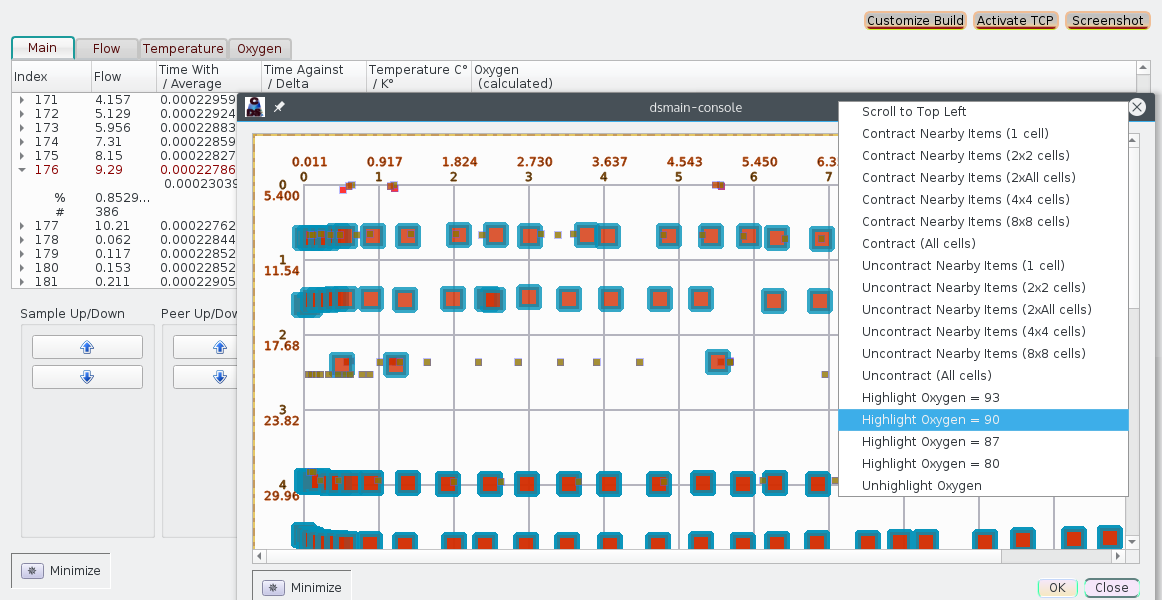
\includegraphics[width=180mm, 
    	trim={0mm 0mm 0mm 0mm},clip]
    	{pics/oxy.png}};
    
\end{tikzpicture}   
\end{figure}




\begin{frame}{\ft{\parbox{22cm}{\vspace{6pt}\centering Using Dataset Applications to Understand 
Experimental Protocols and Research Methods}}}
\vspace{-11em}
\OneQuad
{
\begin{quadblock}{Obtaining Information About Modeling Parameters}
\hspace{1cm}{\parbox{19cm}{\LARGE
\fontseries{b}\selectfont
{
In addition to interactive visualization, 
Dataset Applications are useful pedagogic tools.  Within Dataset Applications, 
modeling units such as statistical parameters 
and record fields are visible in situ within a GUI 
--- identified by labels, buttons, and other interactive 
micro-controls.  As a result, users encounter 
modeling elements in a structured visual-interactive context.  
To help the reader learn more about modeling elements, 
Dataset Applications 
are equipped with several pedagogic features (which are 
shown on the following slides):
\vspace{1em} 


\begin{description}
\item[\curlyquote{About} Dialogs] Brief summaries of research terms and parameters.
\item[XPDF Links] Links back to research articles read in an embedded PDF viewer.
\item[XPDF Enhancements] The XPDF viewer can be customized for each data set 
and included with dataset code, with extra features to integrate article 
or book texts with Dataset Applications.
\end{description}
}
}}
\end{quadblock}
}
\end{frame}


\begin{figure}

\caption{Linking Dataset Applications to Publications}
\label{fig:about}

\begin{tikzpicture}

\node[inner sep=0pt] (x1) at (0,0)
    {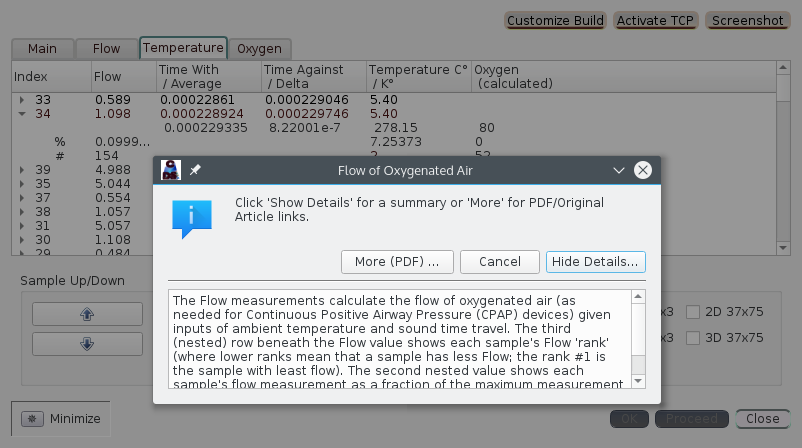
\includegraphics[width=180mm, 
    	trim={0mm 0mm 0mm 0mm},clip]
    	{pics/about.png}};

\end{tikzpicture}    
\end{figure}


\documentclass{article}
%\documentclass{standalone}

\usepackage[active,pdftex,tightpage]{preview}
\usepackage{tikz}

\definecolor{logoYellow}{RGB}{255, 249, 232}
\definecolor{blGreen}{rgb}{.2,.7,.3}
\definecolor{darkRed}{rgb}{.3,0,0}
\newcommand{\sovn}[1]{\color{yellow!20!logoYellow}{{\textbf{#1}}}}

\newcommand{\mybox}[1]{\colorbox{grred!10!darkRed}{\parbox{2mm}{\sovn{#1}}}}

\newcommand{\circled}[1]{{\mybox{#1}}}


\PreviewEnvironment{tikzpicture}

% remove "[demo]" if you want include actual image!!!
\usepackage{graphicx}

\usepackage{tikz}

% LaTeX Overlay Generator - Annotated Figures v0.0.1
% Created with http://ff.cx/latex-overlay-generator/

\definecolor{postBkgColor}{rgb}{.95,.85,.95}
\definecolor{postCommentBkgColor}{rgb}{.85,.85,.95}

\definecolor{grammarArrowColor}{rgb}{.85,.85,.45}

\colorlet{brred}{brown!53!red}
\colorlet{grred}{grammarArrowColor!40!red!60}

\definecolor{logoRed}{rgb}{.3,0,0}
\definecolor{logoPeach}{RGB}{255, 159, 102}
\definecolor{logoCyan}{RGB}{66, 206, 244}
\definecolor{logoBlue}{RGB}{4, 2, 25}

\colorlet{lplr}{logoPeach!40!logoRed}

%%%%%%%%%%%%%%%%%%%%%%%%%%%%%%%%%%%%%%%%%%%%%%%%%%%%%%%%%%%%%%%%%%%%%%
%\annotatedFigureBoxCustom{bottom-left}{top-right}{label}{label-position}{box-color}{label-color}{border-color}{text-color}
\newcommand*\annotatedFigureBoxCustom[8]{\draw[#5,thick,rounded corners] (#1) rectangle (#2);\node at (#4) [fill=#6,thick,shape=circle,draw=#7,inner sep=2pt,font=\sffamily,text=#8] {\textbf{#3}};}
%\annotatedFigureBox{bottom-left}{top-right}{label}{label-position}
\newcommand*\annotatedFigureBox[4]{\annotatedFigureBoxCustom{#1}{#2}{#3}{#4}{lplr}{grred!30!black}{brred}{brred!20}}
\newcommand*\annotatedFigureText[4]{\node[draw=none, anchor=south west, text=#2, inner sep=0, text width=#3\linewidth,font=\sffamily] at (#1){#4};}
\newenvironment {annotatedFigure}[1]{\centering\begin{tikzpicture}
    \node[anchor=south west,inner sep=0] (image) at (0,0) { #1};\begin{scope}[x={(image.south east)},y={(image.north west)}]}{\end{scope}\end{tikzpicture}}
%%%%%%%%%%%%%%%%%%%%%%%%%%%%%%%%%%%%%%%%%%%%%%%%%%%%%%%%%%%%%%%%%%%%%%

\begin{document}

    \begin{figure}[h!t]

        \begin{annotatedFigure}
            {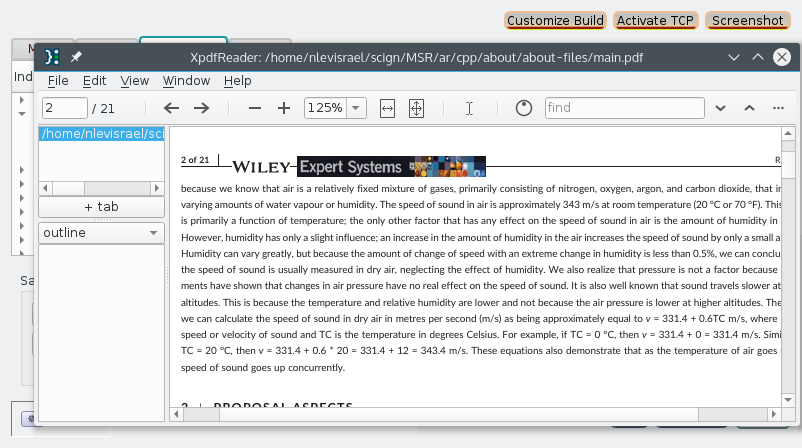
\includegraphics[scale=1]{xpdf.png}}
            
  \node [text width=12.2cm,align=justify,fill=logoCyan!20, draw=logoBlue, 
  draw opacity=0.5,line width=1mm, fill opacity=0.9]
   at (0.3,0.82){\textbf{Each data set can be linked back to an original 
   article or other publication reporting on the data set and 
   experimental results.
   Different parts of the data set can be linked to 
   textual anchors in the publication.  In this example, 
   after viewing a short description of a particular data field 
   inside the Dataset Application, researchers have the option 
   of studying that parameter further by reading at the location 
   in the original publication where the field is introduced or described.  
   The XPDF viewer is compiled as an embedded application 
   within the main Dataset Application and can itself be customized 
   for each data set.}};

            \annotatedFigureBox{0.2,0.12}{0.98,0.65}{1}{0.59,0.665}%            
      %      \annotatedFigureBox{0.222,0.284}{0.3743,0.4934}{B}{0.3743,0.4934}%tr
      %      \annotatedFigureBox{0.555,0.784}{0.6815,0.874}{C}{0.555,0.784}%bl
      %      \annotatedFigureBox{0.557,0.322}{0.8985,0.5269}{D}{0.8985,0.5269}%tr
  
        \end{annotatedFigure}

   %     \caption{Expanded Sample (A)}
    %    \label{fig:teaser}

    \end{figure}

\end{document}




\begin{frame}{\ft{Testing and Fine-Tuning Dataset Applicationss}}
\vspace{-13em}
\OneQuad
{
\begin{quadblock}{Tools for Editors and Developers}
\hspace{1cm}{\parbox{19cm}{\LARGE
\fontseries{b}\selectfont
{
Although ordinary users can explore and visualize 
dsC data sets \curlyquote{Out of the Box}, advanced 
users have many options for customizing their 
build of the application in terms of their specific 
roles and available 3rd-party libraries.  These 
fine-tuning possibilities include:
\vspace{1em} 


\begin{description}
\item[Test Suites] Tools for creating and/or running test suites to 
ensure that the Dataset Application works across platforms.
\item[Data Export] Tools for reusing data in other projects.
\item[External Libraries] Some features like XPDF and 3D graphics 
require libraries that cannot be published with the data set in 
source code form.  Advanced users can slect which of these 
libraries to incoporate into thir version of the 
Dataset Application.
\item[Scripting] Data sets can comoile their own scripting 
environment to automate testing and manipulation of research data.
\item[Networking] Dataset Applications can use an embedded 
TCP server to communicate with other applications, 
enabling multi-application workflows (this is also 
how testing is implemented).

\end{description}
}
}}
\end{quadblock}
}
\end{frame}

\atsp
\begin{frame}{\ft{Config}}

\begin{annotatedFigure}{0pt}{0pt}{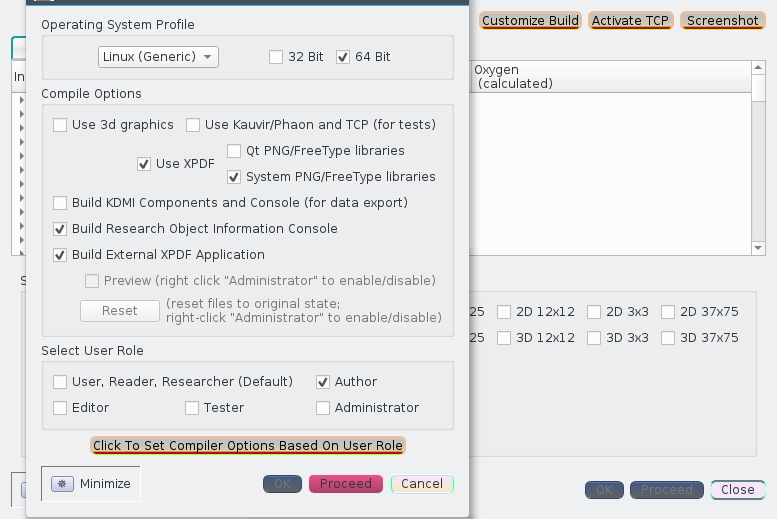
\includegraphics[scale=1]{texs/config.png}}
            
  \node [text width=8.1cm,align=justify,fill=logoCyan!20, draw=logoBlue, 
  draw opacity=0.5,line width=1mm, fill opacity=0.9]
   at (0.79,0.72){\textbf{Using Qt Creator, the Dataset Creator 
   will automatically launch the main Dataset \mbox{Application} 
   with every feature needed in order to \mbox{visualize} 
   and explore the data.  In 
   addition, the data set includes several 
   configurations allowing users to incorporate more specialized 
   or complex features, such as XPDF, test suites, and 
   data export code.  Users can fine-tune which additional 
   features they wish to utilize --- via a separate dialog box 
   \mbox{(\circled{1} and \circled{2})} --- to create a customized build of the 
   main Dataset Application and supplemental executables.}};

  \annotatedFigureBox{0.61,0.93}{0.75,0.982}{1}{0.75,0.922}%
            \annotatedFigureBox{0.033,0.12}{0.58,0.97}{2}{0.58,0.97}%            
      %      \annotatedFigureBox{0.222,0.284}{0.3743,0.4934}{B}{0.3743,0.4934}%tr
      %      \annotatedFigureBox{0.555,0.784}{0.6815,0.874}{C}{0.555,0.784}%bl
      %      \annotatedFigureBox{0.557,0.322}{0.8985,0.5269}{D}{0.8985,0.5269}%tr
    \node [text width=7cm,align=justify,fill=logoCyan!20, draw=logoBlue, 
    draw opacity=0.5,line width=1mm, fill opacity=0.9]
     at (0.778,0.3){\textbf{The Dataset Creator 
     also recognizes distinct ``roles" (\circled{2}), including 
     general readers, authors, those who double-check the 
     main Dataset Application via a test suite, and those 
     who design the test suite and write dataset code overall 
     (dubbed ``Administrators").}};
  
   \annotatedFigureBox{0.05,0.16}{0.57,0.35}{2}{0.57,0.35}
        
      
  
        \end{annotatedFigure}

   %     \caption{Expanded Sample (A)}
    %    \label{fig:teaser}

    \end{frame}




    \begin{frame}{\ft{Testing}}

        \begin{annotatedFigure}{0pt}{0pt}
            {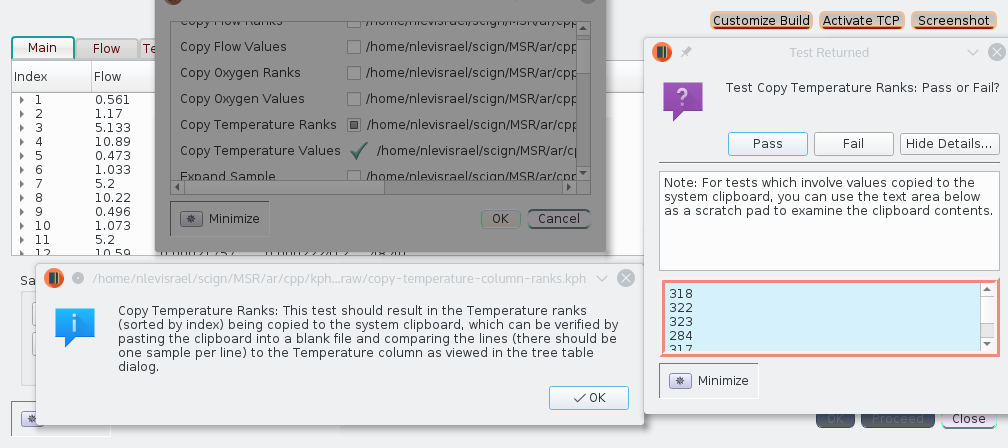
\includegraphics[scale=1]{texs/testing.png}}
            
  \node [text width=20cm,align=justify,fill=logoCyan!20, draw=logoBlue, 
  draw opacity=0.5,line width=1mm, fill opacity=0.9]
   at (0.38,0.93){\textbf{Dataset Creator includes a sophisticated 
   framework for building and running test suites to 
   ensure that raw data is processed correctly and that 
   User Interface components work properly on different 
   Operating System platforms.  This includes 
   a separate testing application that sends instructions 
   to the main Dataset Application via TCP (\circled{1}).}};

  \annotatedFigureBox{0.81,0.93}{0.903,0.982}{1}{0.903,0.935}%
  
  
   \node [text width=4cm,align=justify,fill=logoCyan!20, draw=logoBlue, 
   draw opacity=0.5,line width=1mm, fill opacity=0.9]
    at (0.08,0.64){\textbf{The testing application has several 
    features to facilitate running tests, including 
    options to repeat tests, mark success or failure (\circled{2}), and 
    examine the system clipboard (\circled{3}).}};
 
  \annotatedFigureBox{0.17,0.63}{0.37,0.685}{2}{0.37,0.63}
   \annotatedFigureBox{0.651,0.113}{0.995,0.86}{3}{0.892,0.86}% 

   \node [text width=11cm,align=justify,fill=logoCyan!20, draw=logoBlue, 
   draw opacity=0.5,line width=1mm, fill opacity=0.9]
    at (0.26,0.09){\textbf{Testers can 
    also read a description of each test (\circled{4}),  
    and view the scripts used to ceate them.}};
 
  \annotatedFigureBox{0.05,0.16}{0.62,0.325}{4}{0.62,0.19}
  
      %      \annotatedFigureBox{0.222,0.284}{0.3743,0.4934}{B}{0.3743,0.4934}%tr
      %      \annotatedFigureBox{0.555,0.784}{0.6815,0.874}{C}{0.555,0.784}%bl
      %      \annotatedFigureBox{0.557,0.322}{0.8985,0.5269}{D}{0.8985,0.5269}%tr
  
        \end{annotatedFigure}

    \end{frame}




\atsp
\begin{frame}{\ft{Features of Dataset Applications for Books}}
\vspace{-13em}
\hspace*{6pt}\OneQuad
{
\begin{quadblock}{Datasets Ccompiled From Book Examples}
\hspace{1cm}{\parbox{19cm}{\LARGE
\fontseries{b}\selectfont
{
The remaining screenshots demonstrate how data sets can be 
used even outside of a lab contxt generating 
experiment data.  The pictured data set represents a corpus 
of linguistic examples mined from Wiley's \textit{Blackwell Handbook 
of Pragmatics}.  Creating data sets from book-length publications 
can encompass several steps:
\vspace{1em} 
\begin{description}
\item[Text Mining] In the case of linguistics, this involves 
locating example sentences within linguistics texts and 
storing them as an independent corpus.
\item[Canonical Formatting] If possible, linguistics 
texts should be annotated so that extracting exmples can be automated.
\item[Annotation] Linguistic corpuses are often annotated 
to identify structural details, beyond raw text, in 
each sample.
\end{description}
}
}}
\end{quadblock}
}
\end{frame}

    \begin{frame}{\ft{Creating a Data Set from a Book}}
\section{Group 2: Creating a Data Set from a Book}

        \begin{annotatedFigure}{0pt}{0pt}
            {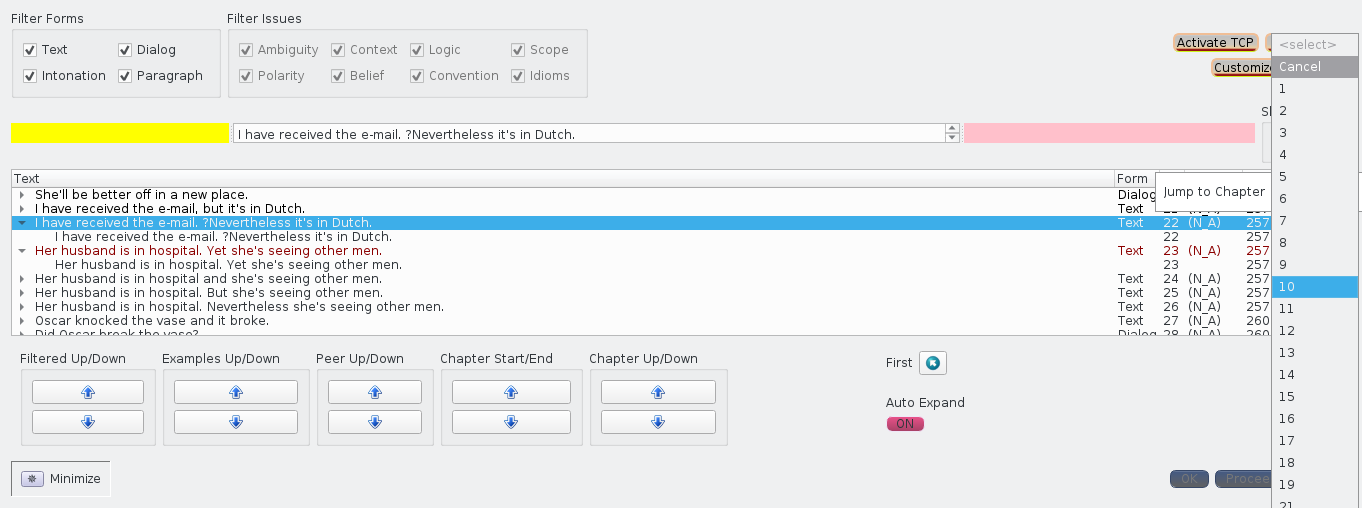
\includegraphics[scale=.86]{texs/chapter.png}}
            
  \node [text width=12.5cm,align=justify,fill=logoCyan!20, draw=logoBlue, 
  draw opacity=0.5,line width=1mm, fill opacity=0.9]
   at (0.49,0.6){\textbf{This screenshow shows 
   a linguistics dataset that illustrates several \mbox{advanced} 
   interactive feaures made possible by the Dataset \mbox{Creator}'s 
   Qt-based front-end technology.  Useful features include context 
   menus \mbox{embedded} with drop-down selections (\circled{1}) and 
   button/checkbox groups for filtered scrolling through 
   a list of samples (\circled{2} and \circled{3}).}};
    
            \annotatedFigureBox{0.93,0.02}{0.985,0.945}{1}{0.985,0.945}%                
            \annotatedFigureBox{0.005,0.82}{0.43,0.98}{2}{0.43,0.82}%
         
            \annotatedFigureBox{0.01,0.1}{0.55,0.334}{3}{0.55,0.334}            
            
      %      \annotatedFigureBox{0.222,0.284}{0.3743,0.4934}{B}{0.3743,0.4934}%tr
      %      \annotatedFigureBox{0.555,0.784}{0.6815,0.874}{C}{0.555,0.784}%bl
      %      \annotatedFigureBox{0.557,0.322}{0.8985,0.5269}{D}{0.8985,0.5269}%tr
  

  
        \end{annotatedFigure}

   %     \caption{Expanded Sample (A)}
    %    \label{fig:teaser}

    \end{frame}


\atsptt
\begin{frame}{\ft{Interacting with Data Samples}}
\section{Group 2: Interacting with Data Samples}
 \vspace{16pt}
        \begin{annotatedFigure}{30pt}{2pt}
            {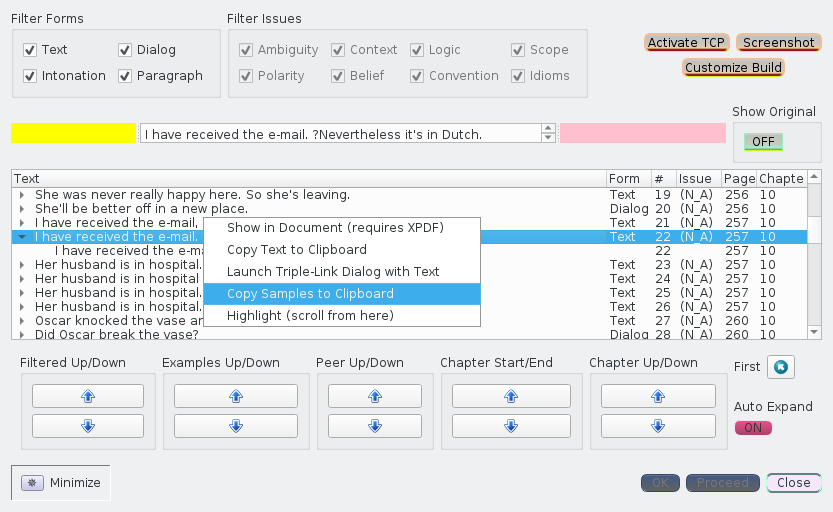
\includegraphics[scale=1.2]{texs/lingcopy.png}}
            
  \node [text width=10cm,inner sep=14pt,align=justify,fill=logoCyan!20, %draw=logoBlue, 
  %draw opacity=0.5,
  %line width=1mm, 
  fill opacity=0.9,
  top color=blue!20,
  bottom color=blue!40,
  rounded corners=6pt]
   at (0.29,0.82){\annfont\textbf{The linguistic samples comprising 
   this data set are all example sentences, phrases, 
   or dialog-snippets that are used, in the \textit{Blackwell 
   Handbook of Pragmatics}, as expository samples for 
   case-studies of various linguistic phenomenon and 
   pragmatics, semantics, and grammatical theories.}};
    
%notatedFigureBox{0.93,0.02}{0.985,0.945}{1}{0.985,0.945}%                
%\annotatedFigureBox{0.005,0.82}{0.43,0.98}{2}{0.43,0.82}%
%\annotatedFigureBox{0.01,0.1}{0.55,0.334}{3}{0.55,0.334}            
            
      %      \annotatedFigureBox{0.222,0.284}{0.3743,0.4934}{B}{0.3743,0.4934}%tr
      %      \annotatedFigureBox{0.555,0.784}{0.6815,0.874}{C}{0.555,0.784}%bl
      %      \annotatedFigureBox{0.557,0.322}{0.8985,0.5269}{D}{0.8985,0.5269}%tr
  

  
        \end{annotatedFigure}

\end{frame}




   \begin{frame}{\ft{Linking Back to the Book}}
\section{Group 2: Linking Back to the Book}

        \begin{annotatedFigure}{0pt}{0pt}
            {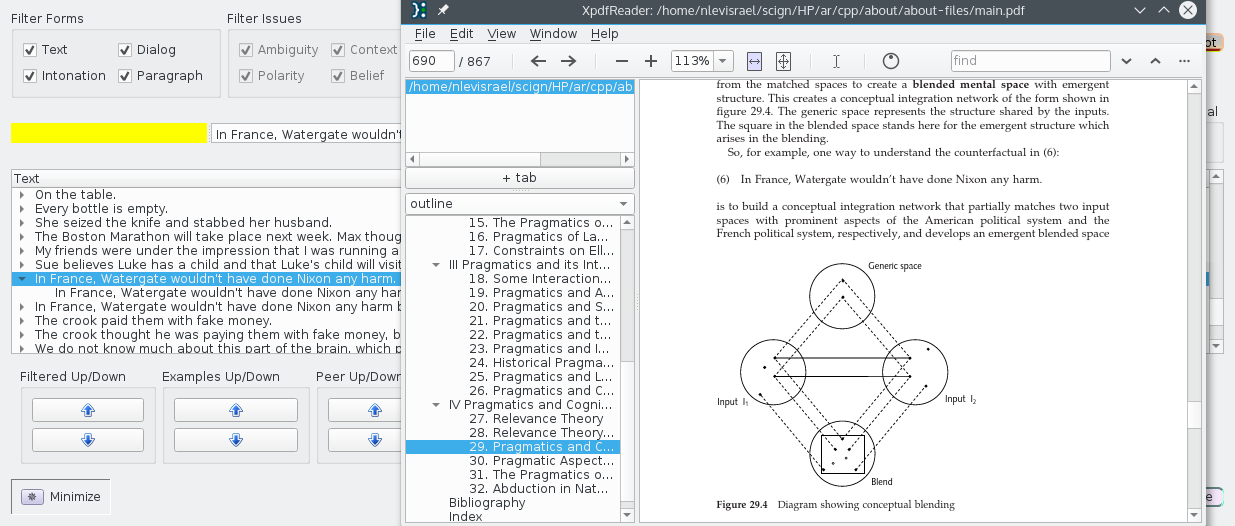
\includegraphics[scale=1]{texs/nixon.png}}
            
  \node [text width=6.7cm,inner sep=4pt,align=justify,
  bottom color=brown!80!purple,
  top color=white, %top color=blue!40!cyan, 
  shading angle=310, 
  %fill=logoCyan!20, draw=logoBlue, 
  %draw opacity=0.5,
  %line width=1mm, 
  %fill opacity=0.9
  ]
   at (0.45,0.713){\vspace{-6pt}\cframedboxyellow{\annfont\textbf{After browsing through the data set, 
   users can link back to the original text to 
   see the current author's discussion of particular examples.}}};
    
%notatedFigureBox{0.93,0.02}{0.985,0.945}{1}{0.985,0.945}%                
%\annotatedFigureBox{0.005,0.82}{0.43,0.98}{2}{0.43,0.82}%
%\annotatedFigureBox{0.01,0.1}{0.55,0.334}{3}{0.55,0.334}            
            
      %      \annotatedFigureBox{0.222,0.284}{0.3743,0.4934}{B}{0.3743,0.4934}%tr
      %      \annotatedFigureBox{0.555,0.784}{0.6815,0.874}{C}{0.555,0.784}%bl
      %      \annotatedFigureBox{0.557,0.322}{0.8985,0.5269}{D}{0.8985,0.5269}%tr
  

  
        \end{annotatedFigure}

    \end{frame}



\atsp
\begin{frame}{\ft{A Linguistics Annotation System}}
\vspace{-13em}
\hspace*{6pt}\OneQuad
{
\begin{quadblock}{Tools to Facilitate Annotating Linguistic Corpora}
\hspace{1cm}{\parbox{19cm}{\LARGE
\fontseries{b}\selectfont
{The final three screenshots show an example of how a 
custom-signd application can 
facilotat the task of building 
an annotated corpus from a linguistics text.  
The components demonstrated here enable 
several strategies (which can be combined) for dscribing 
parsing structures and the logical 
composition of language samples:
\vspace{1em} 
\begin{description}
\item[S-Expressions] Representing linguistic units as 
semantic and syntactic transformations 
triggered by words assigned to \curlyquote{functional} 
types.
\item[Deepndency Grammar] Representing phrase structures viabinter-word 
syntactic relationships.
\item[Link Grammar] Representing linguistic structure via connectors 
internal to each word-sense.  Inter-word links are activatd when 
each word in the pair has a connector compatible with the 
other word's connector.  Intuitively, a connctor represents 
how one word's meaning or grammatic contribution can 
be \curlyquote{completed} by linking to a separate word.
\end{description}
}
}}
\end{quadblock}
}
\end{frame}


    \begin{frame}{\ft{Building Parsing Models}}
\section{Group 1: Building Parsing Models}

        \begin{annotatedFigure}{10pt}{0pt}{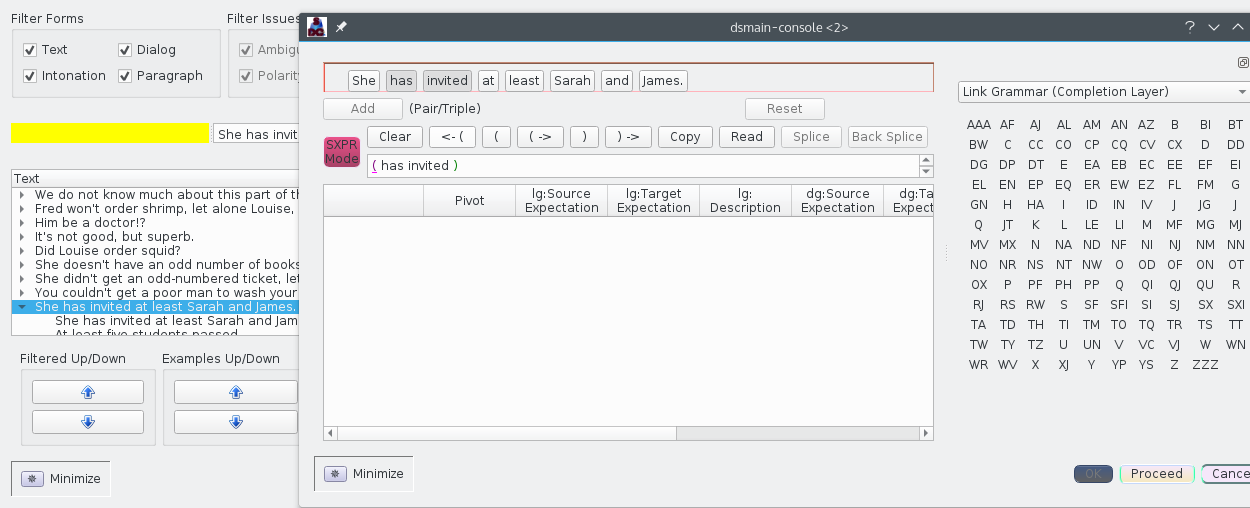
\includegraphics[trim={3.cm 0 0 0},clip]{texs/sxpr.png}}  
        	
      \node [text width=8cm,inner sep=14pt,align=justify,fill=logoCyan!20, draw=logoBlue, 
      draw opacity=0.5,line width=1mm, fill opacity=0.9]
      at (0.41,0.36){\annfont\textbf{The main Dataset Application 
      		for the demo Linguistics data set includes a 
      		distinct window for building annotations on language examples. 
      		Features of this component include an entry area 
      		for building S-Expression models of sentences with visual cues 
      		such as parenthesis-matching color highlights (\circled{1})
      		and sidebars where users can add inter-word annotations using 
      		relations drawn from Link Grammar and 
      		CoNLL-U Dependency Grammar (\circled{2}).}};
          	
 \annotatedFigureBox{0.221,0.655}{0.323,0.696}{1}{0.323,0.696}%
 
 \annotatedFigureBox{0.74,0.27}{0.9985,0.85}{2}{0.76,0.85}%
 
        \end{annotatedFigure}


\end{frame}


    \begin{frame}{\ft{Using Dock Widgets For Flexible Layout}}
\section{Group 1: Using Dock Widgets For Flexible Layout}

        \begin{annotatedFigure}{0pt}{0pt}
            {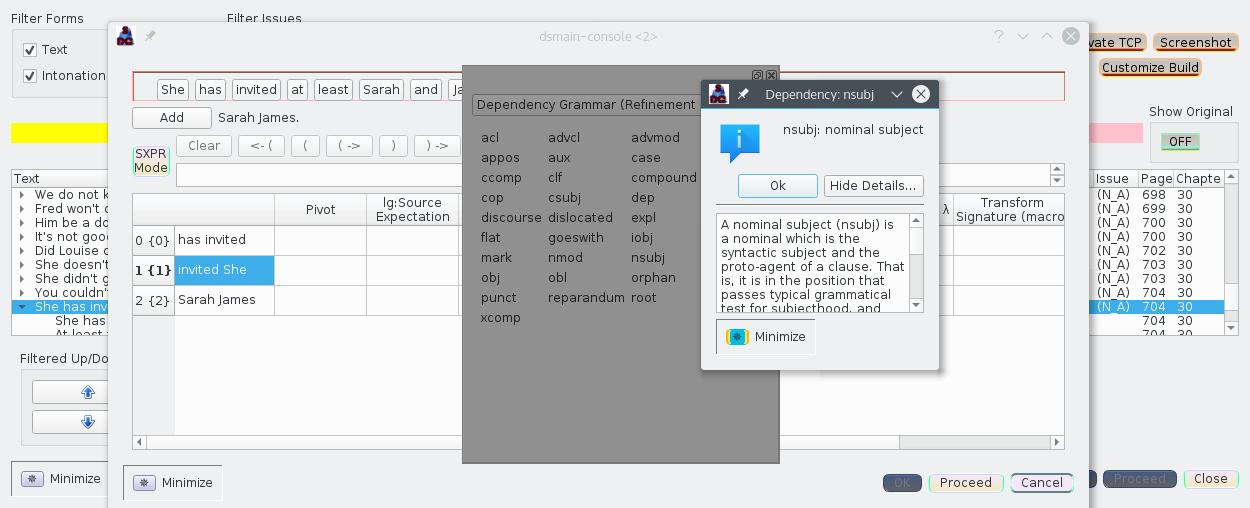
\includegraphics[scale=1]{texs/float.png}}
            
  \node [text width=7cm,inner sep=14pt,align=justify,fill=logoCyan!20, draw=logoBlue, 
  draw opacity=0.5,line width=1mm, fill opacity=0.9]
   at (0.25,0.73){\annfont\textbf{The 
   list of link/dependency relations is also isolated 
   as a ``dock widget" that may be dragged to float 
   above the other application windows  (\circled{1}), 
   or ``docked" at different positions (left or right) 
   on its parent window.  
   This screenshot also shows a dialog 
   box used for a precis of the individual 
   CoNLL-U (Conference on Natural 
   Language Learning - Universal) and Link
   Grammar relations (\circled{2}).}};


\annotatedFigureBox{0.37,0.23}{0.75,0.88}{1}{0.37,0.88}%                
\annotatedFigureBox{0.564,0.3}{0.75,0.84}{2}{0.564,0.84}%
%\annotatedFigureBox{0.01,0.1}{0.55,0.334}{3}{0.55,0.334}            
            
      %      \annotatedFigureBox{0.222,0.284}{0.3743,0.4934}{B}{0.3743,0.4934}%tr
      %      \annotatedFigureBox{0.555,0.784}{0.6815,0.874}{C}{0.555,0.784}%bl
      %      \annotatedFigureBox{0.557,0.322}{0.8985,0.5269}{D}{0.8985,0.5269}%tr
  

  
        \end{annotatedFigure}

\end{frame}


\atsptt
    \begin{frame}{\ft{Link and Dependency Grammar Annotations}}
\section{Group 2: Link and Dependency Grammar Annotations}

        \begin{annotatedFigure}{0pt}{0pt}
            {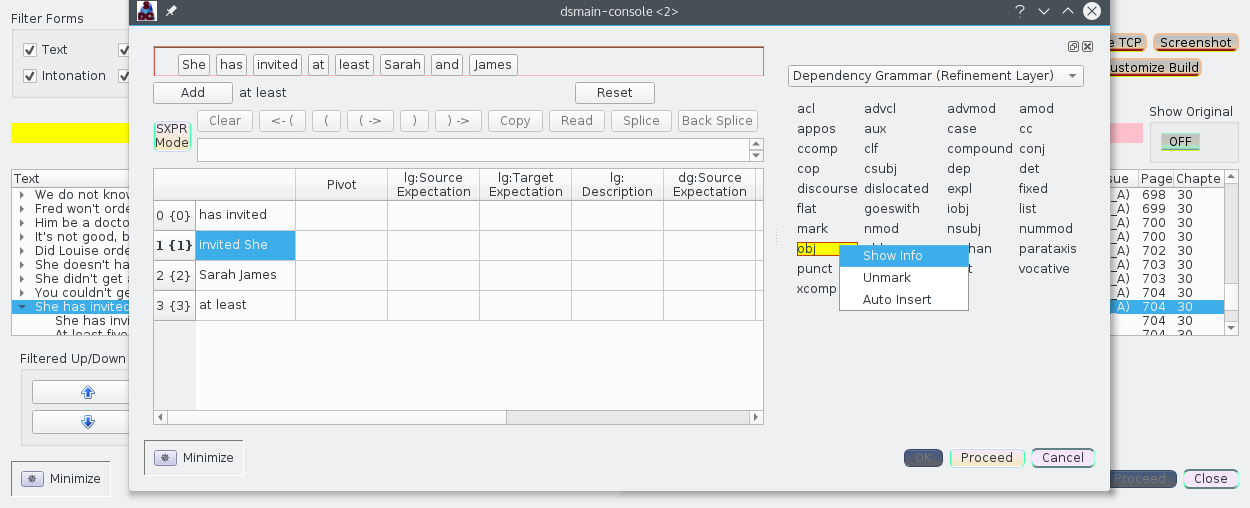
\includegraphics[scale=1]{texs/trilink.png}}
            
  \node [text width=7cm,inner sep=14pt,align=justify,%fill=logoCyan!20, draw=logoBlue, 
  draw opacity=0.9,line width=2mm, fill opacity=0.9,
  draw = logoCyan!50!brown,
  top color=brown!20,text=black,
  bottom color=logoCyan!2,
  rounded corners=6pt]
   at (0.41,0.39){\annfont\textbf{Users can select word-pairs 
   from samples being annotated and then identify 
   the relationship between the selected words, as understood 
   according to Link or Dependency Grammars.  The 
   list of link/dependency relations provides 
   an interface to research and read overviews about the 
   relationships.}};

\curicon{0.77}{0.48}


%\annotatedFigureBox{0.93,0.02}{0.985,0.945}{1}{0.985,0.945}%                
%\annotatedFigureBox{0.005,0.82}{0.43,0.98}{2}{0.43,0.82}%
%\annotatedFigureBox{0.01,0.1}{0.55,0.334}{3}{0.55,0.334}            
            
      %      \annotatedFigureBox{0.222,0.284}{0.3743,0.4934}{B}{0.3743,0.4934}%tr
      %      \annotatedFigureBox{0.555,0.784}{0.6815,0.874}{C}{0.555,0.784}%bl
      %      \annotatedFigureBox{0.557,0.322}{0.8985,0.5269}{D}{0.8985,0.5269}%tr
  

  
        \end{annotatedFigure}

\end{frame}


%{
%	\setbeamercolor{background canvas}{bg=}
%\part{ScreenShots}		

%\section{Group_1-1-intro}\begin{frame}{\ft{Features of dsC}}
%\includepdf[pages=1]{Group_1-1-intro.pdf}
%\end{frame}

%\section{Group_1-1}\begin{frame}{\ft{Conventional Spreadsheet}}
%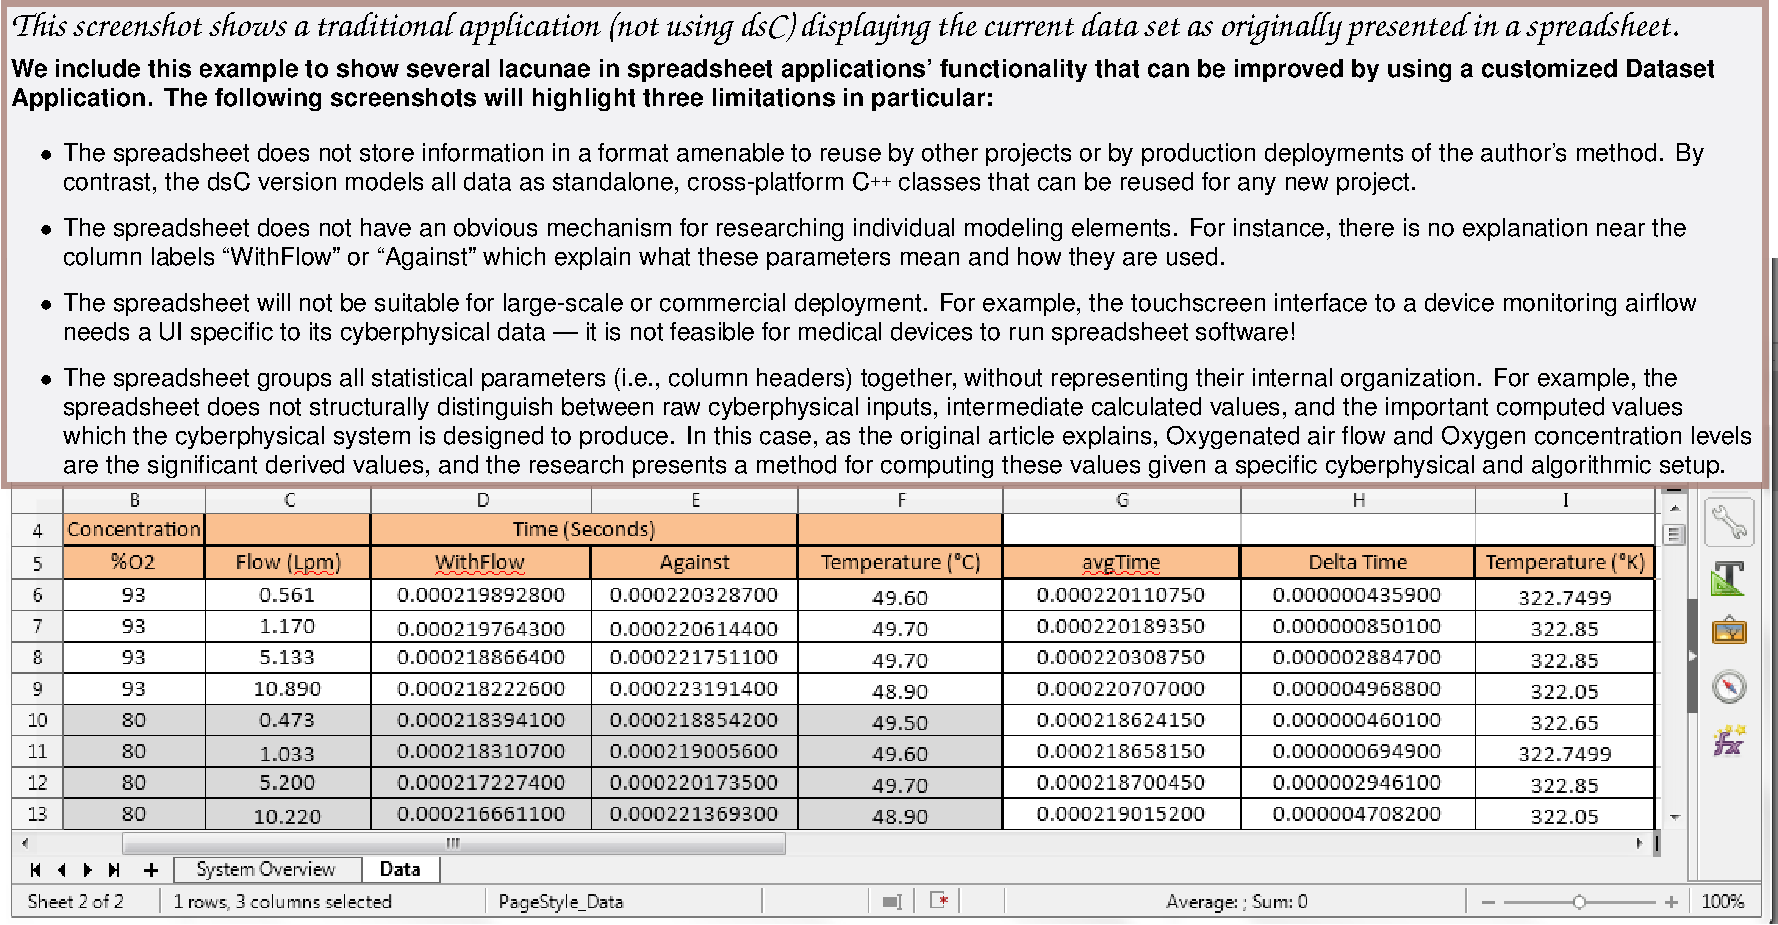
\includepdf[pages=1]{Group_1-1-OriginalSpreadsheet.pdf}
%\end{frame}

%\section{Group_1-2}\begin{frame}{\ft{Tree Widget}}
%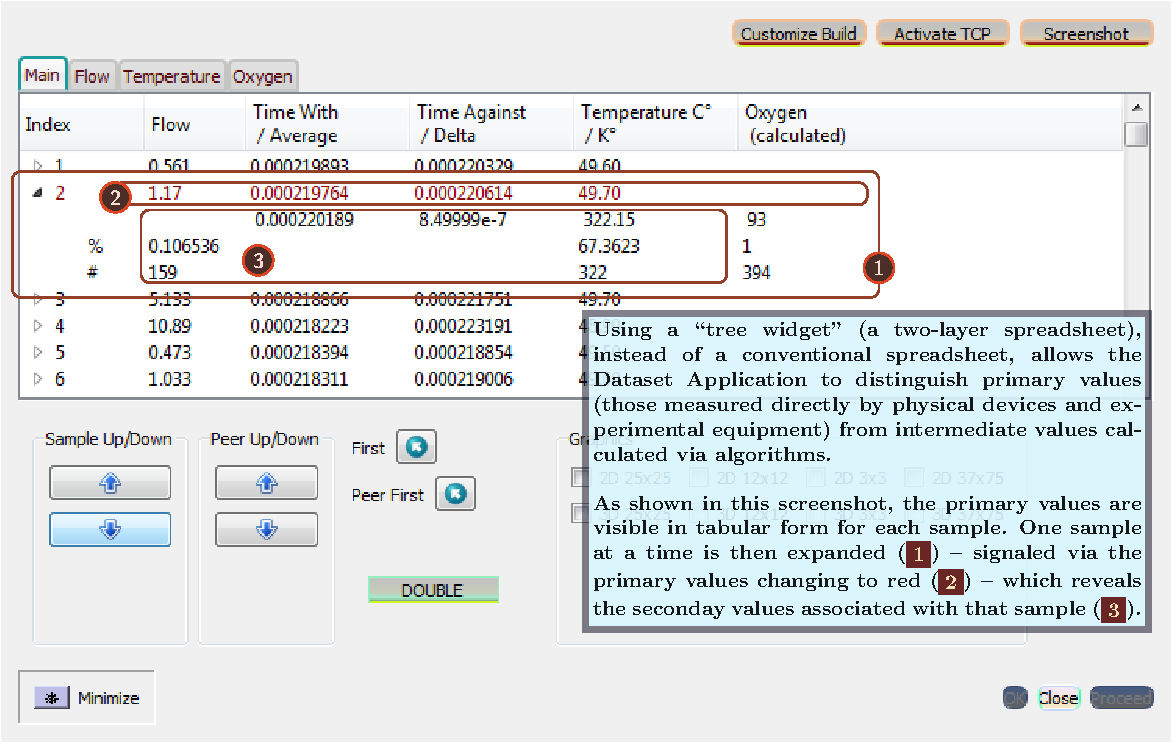
\includepdf[pages=1]{Group_1-2-InitialApplicationWindow.pdf}
%\end{frame}

%\section{Group_1-3}\begin{frame}{\ft{Tree Widget}}
%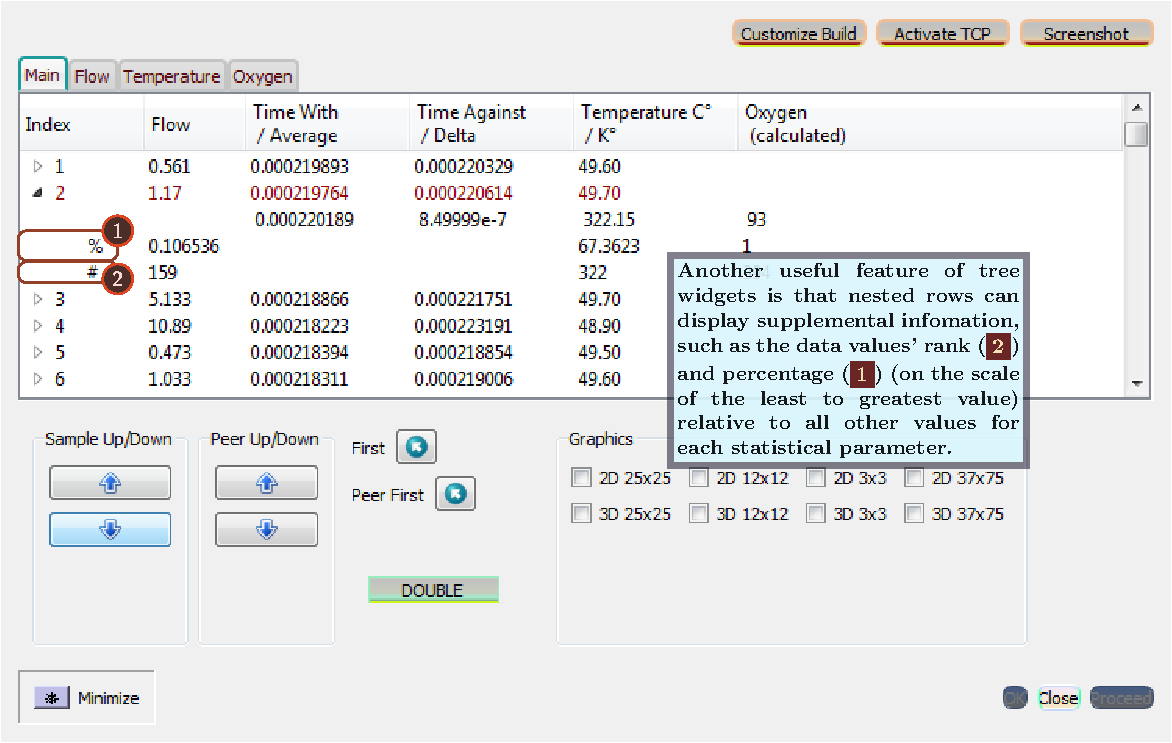
\includepdf[pages=1]{Group_1-3-MoreTreeWidgetFeatures.pdf}
%\end{frame}

%\section{Group_1-4}\begin{frame}{\ft{Tree Widget}}
%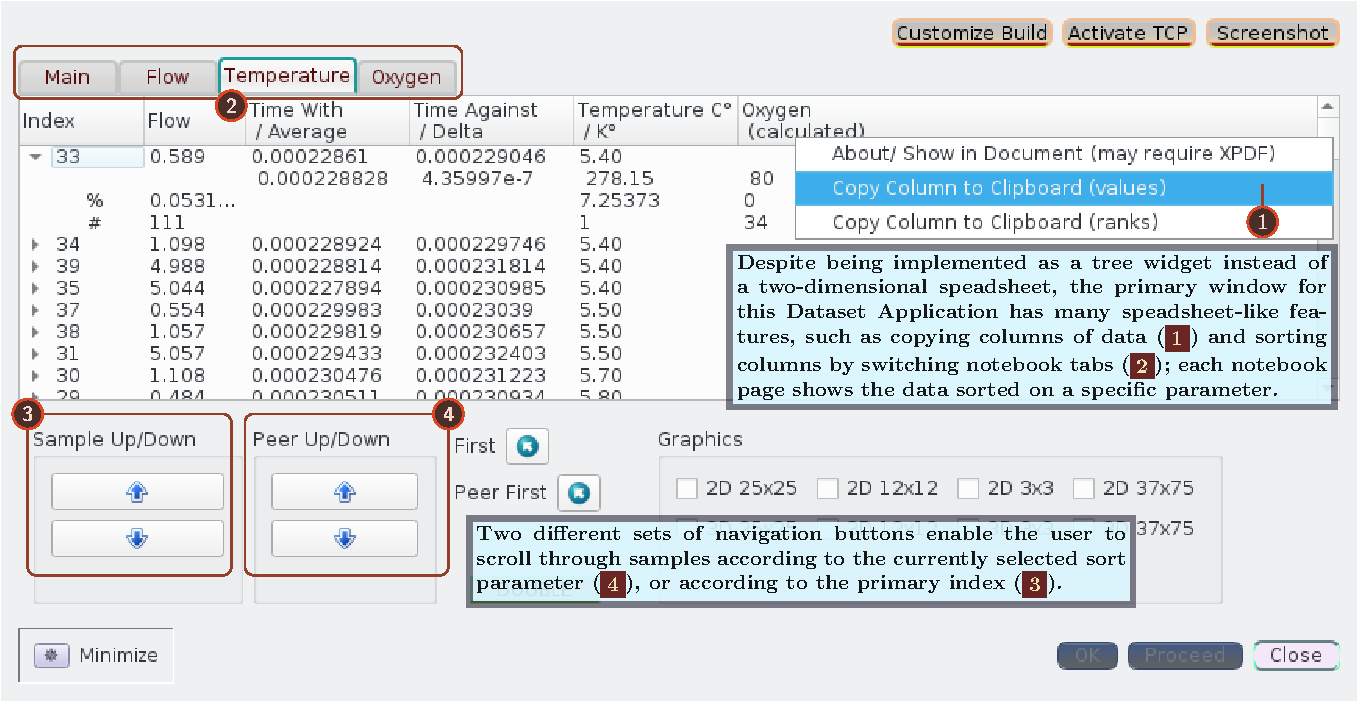
\includepdf[pages=1]{Group_1-4-InteractingWithTheMainWindow.pdf}
%\end{frame}

%\section{Group_1-5}\begin{frame}{\ft{Tree Widget}}
%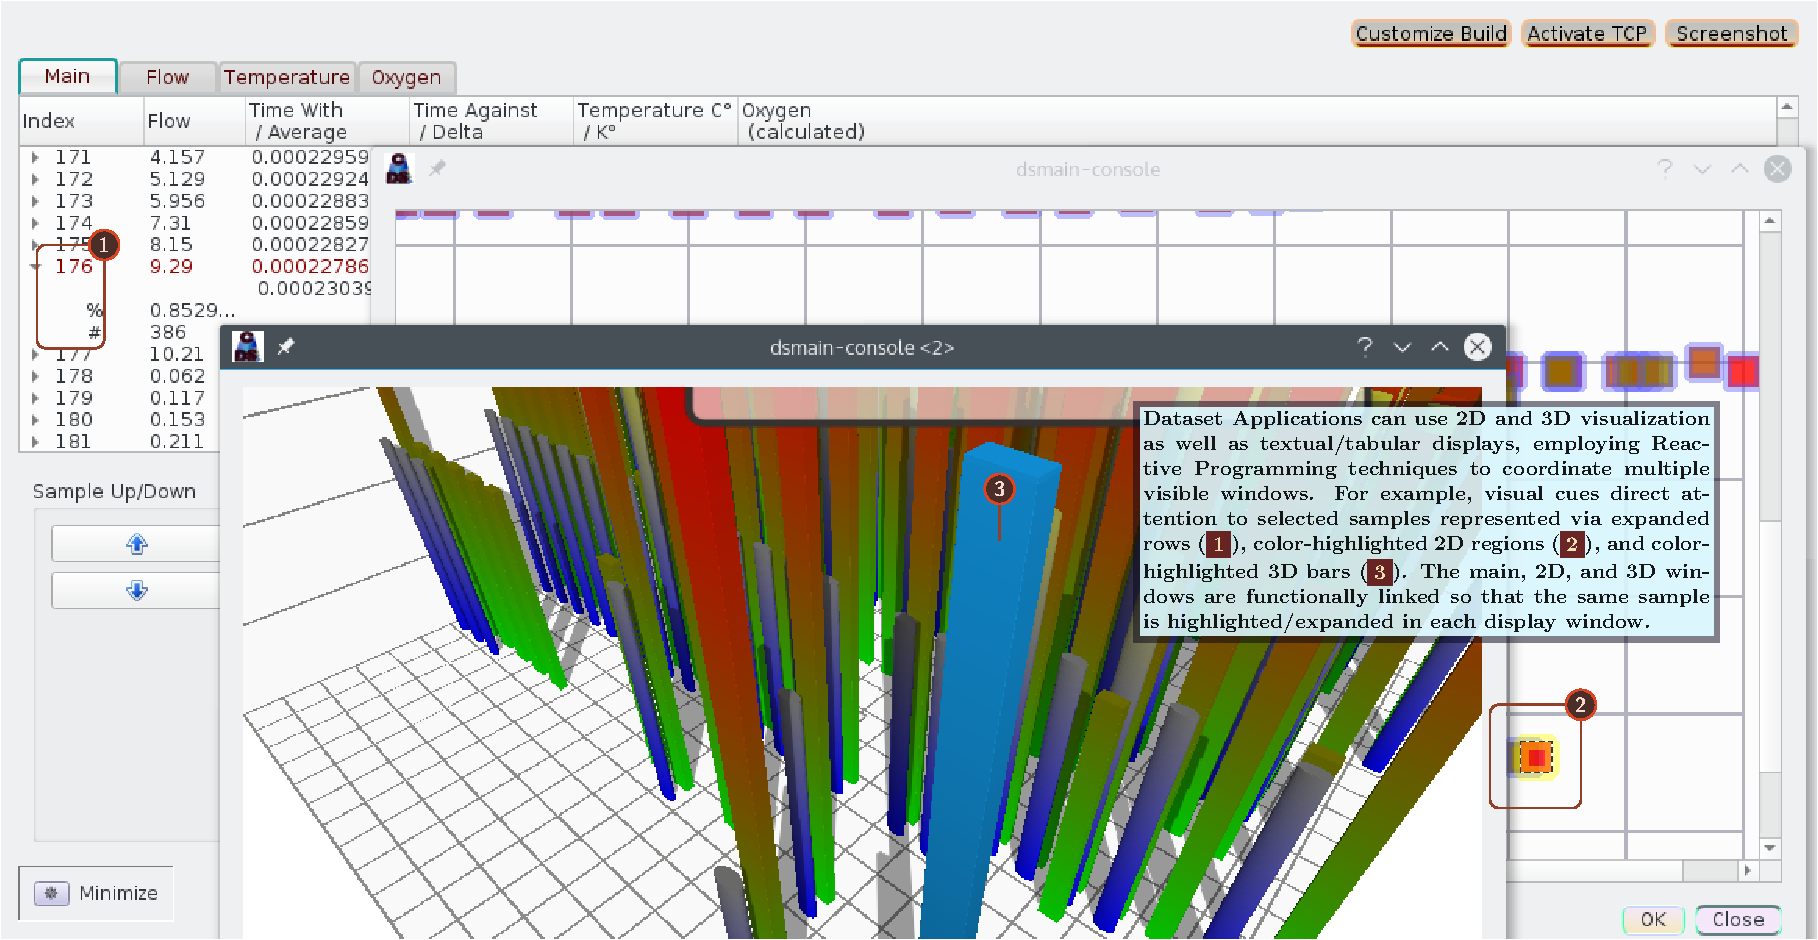
\includepdf[pages=1]{Group_1-5-CoordinatedDataVisualization.pdf}
%\end{frame}

%\section{Group_1-6}\begin{frame}{\ft{Tree Widget}}
%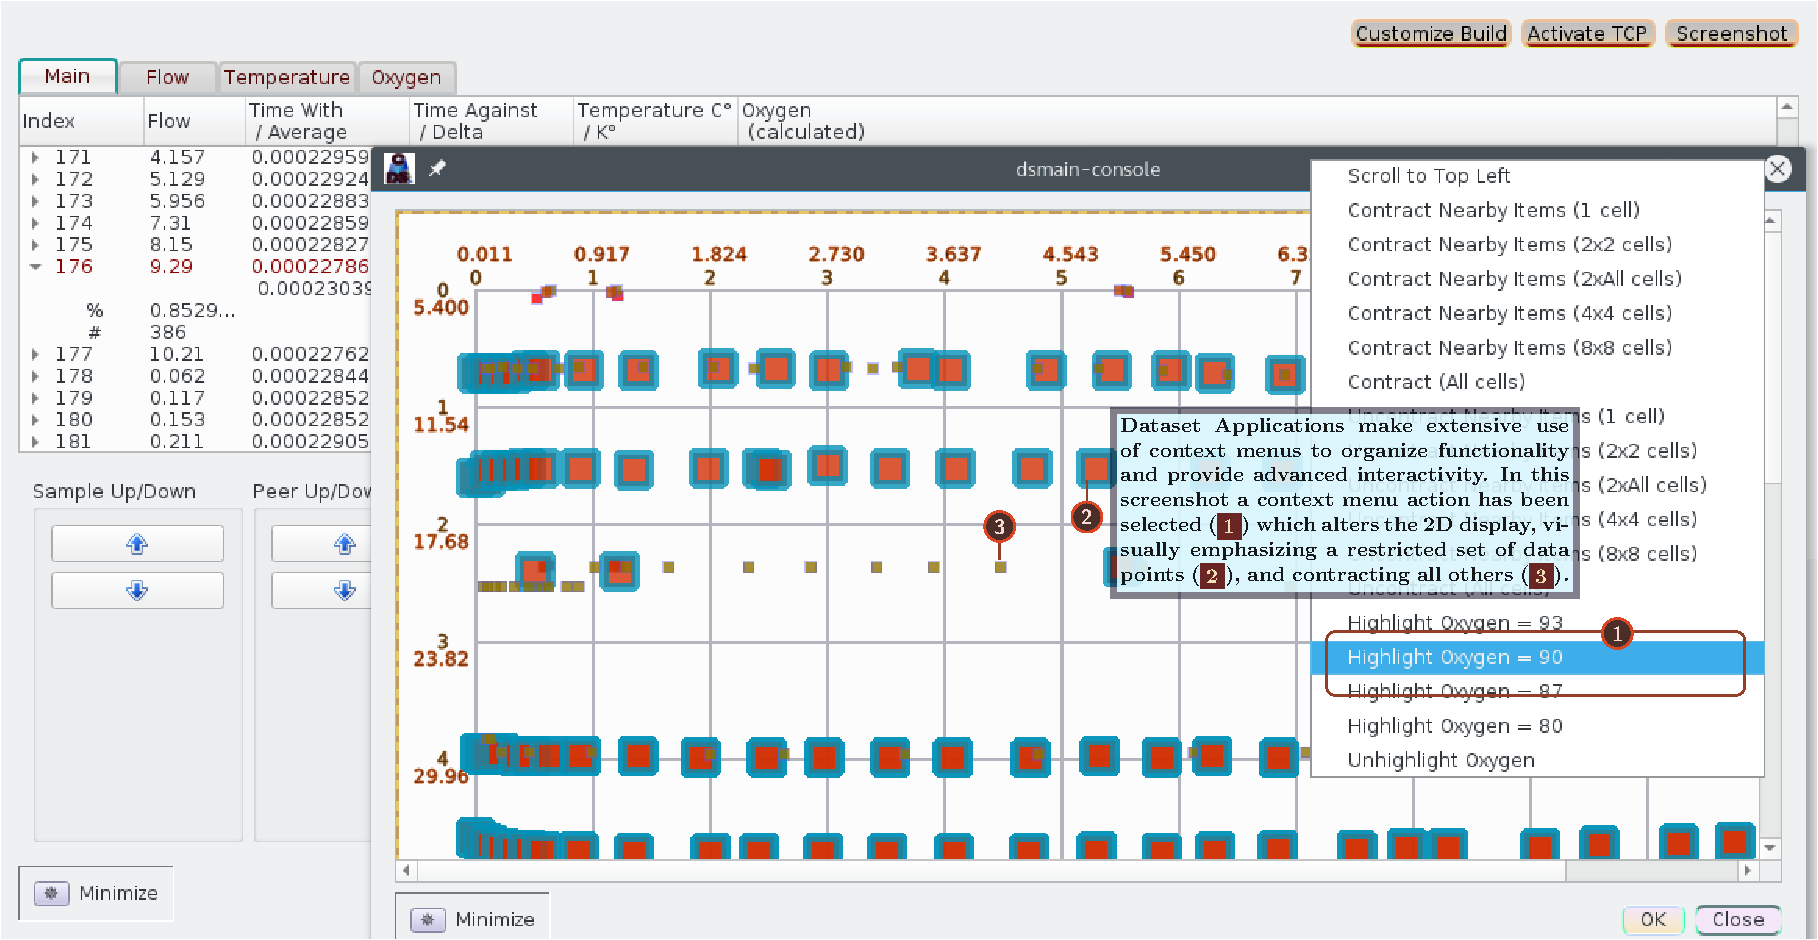
\includepdf[pages=1]{Group_1-6-InteractingWithTheVisuals.pdf}
%\end{frame}

%\section{Group_1-7-intro}\begin{frame}{\ft{Tree Widget}}
%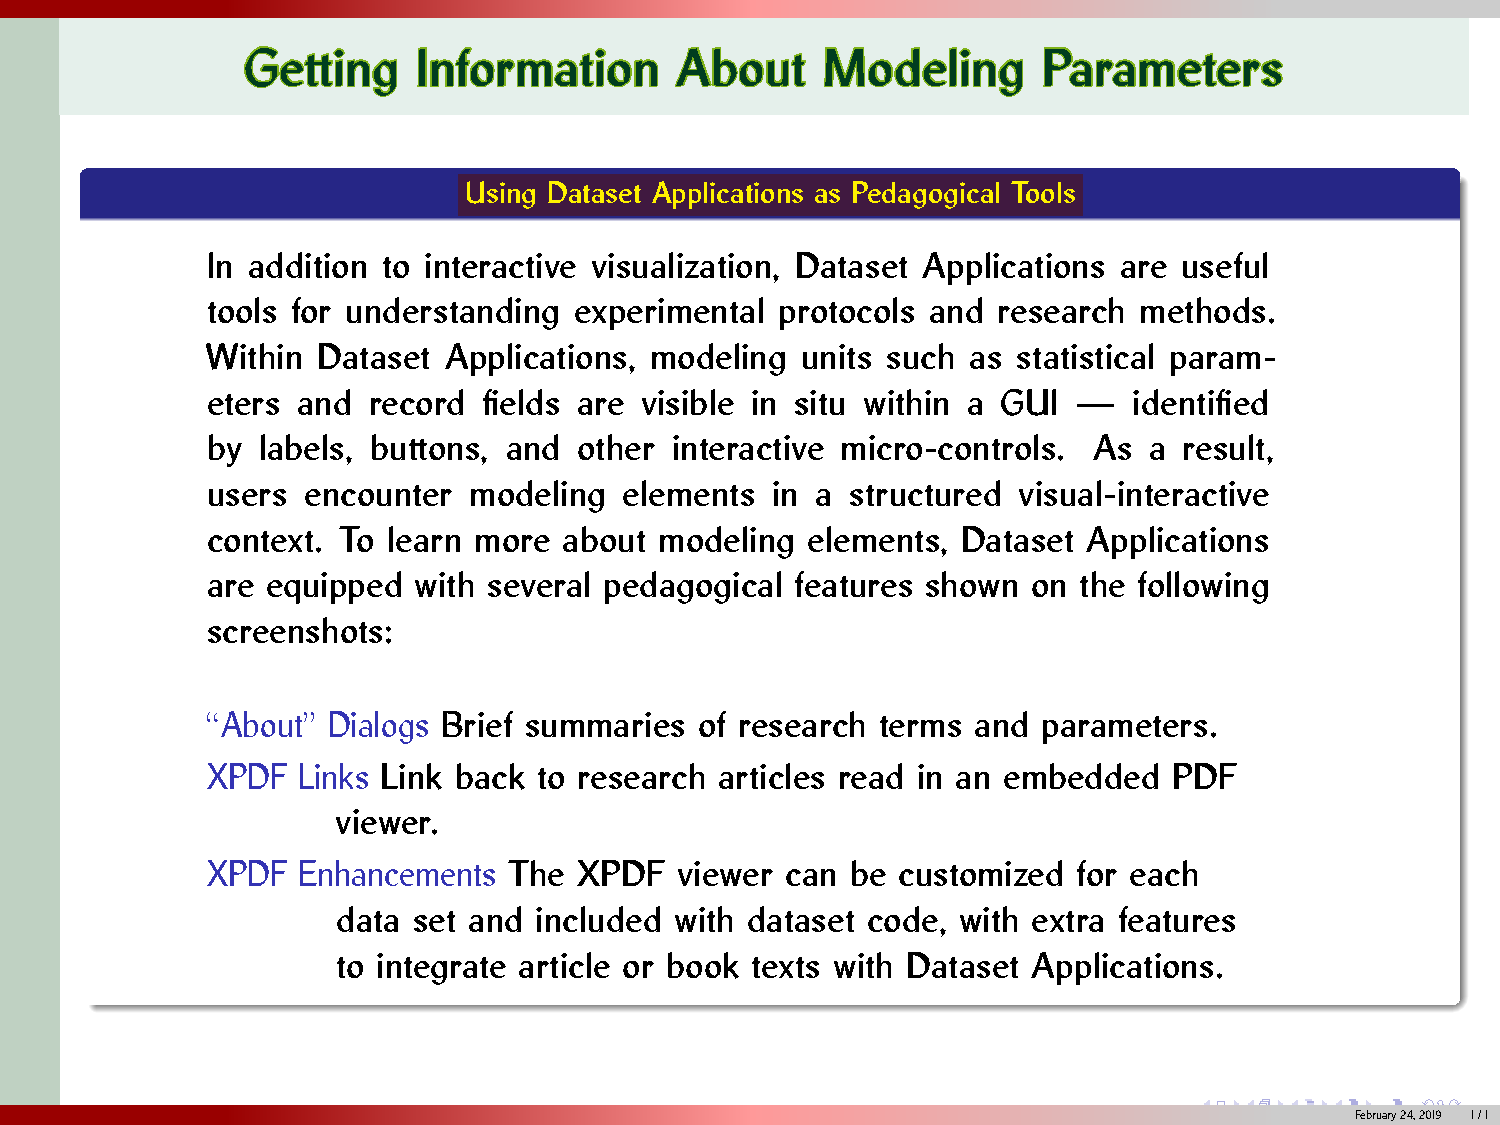
\includepdf[pages=1]{Group_1-7_intro.pdf}
%\end{frame}

%\section{Group_1-7}\begin{frame}{\ft{Tree Widget}}
%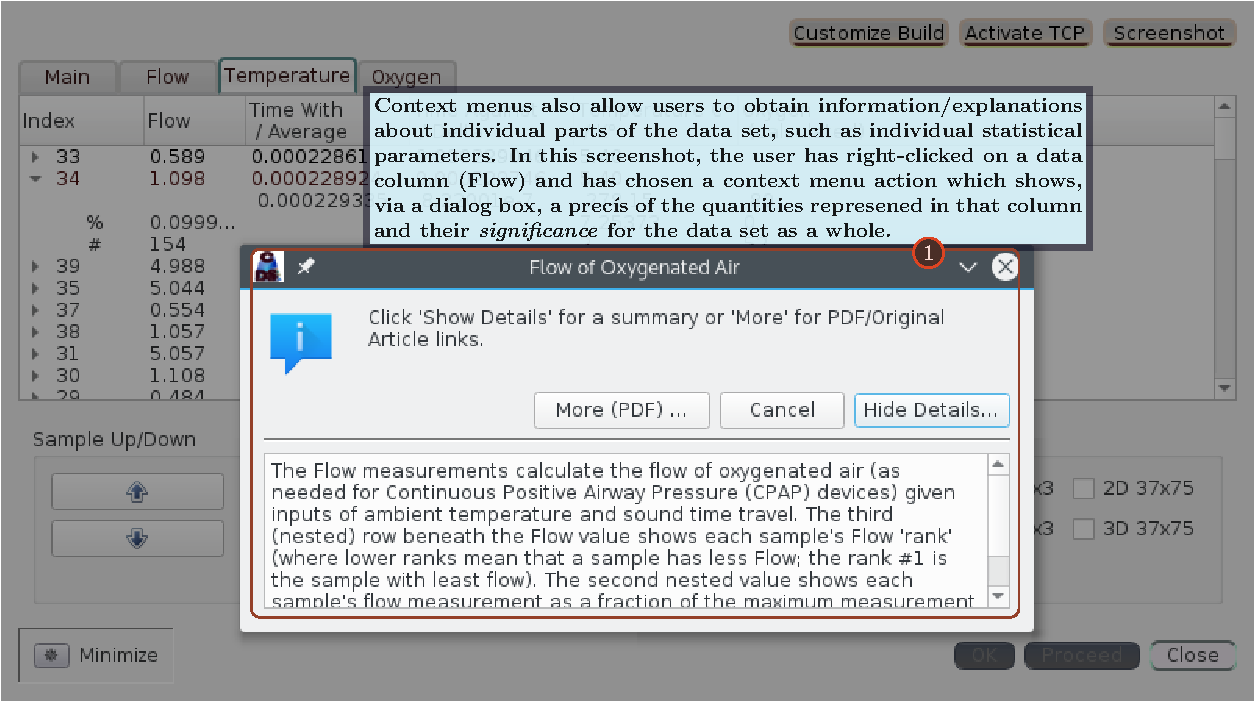
\includepdf[pages=1]{Group_1-7-ObtainingInformationAboutParameters.pdf}
%\end{frame}

%\section{Group_1-8}\begin{frame}{\ft{Tree Widget}}
%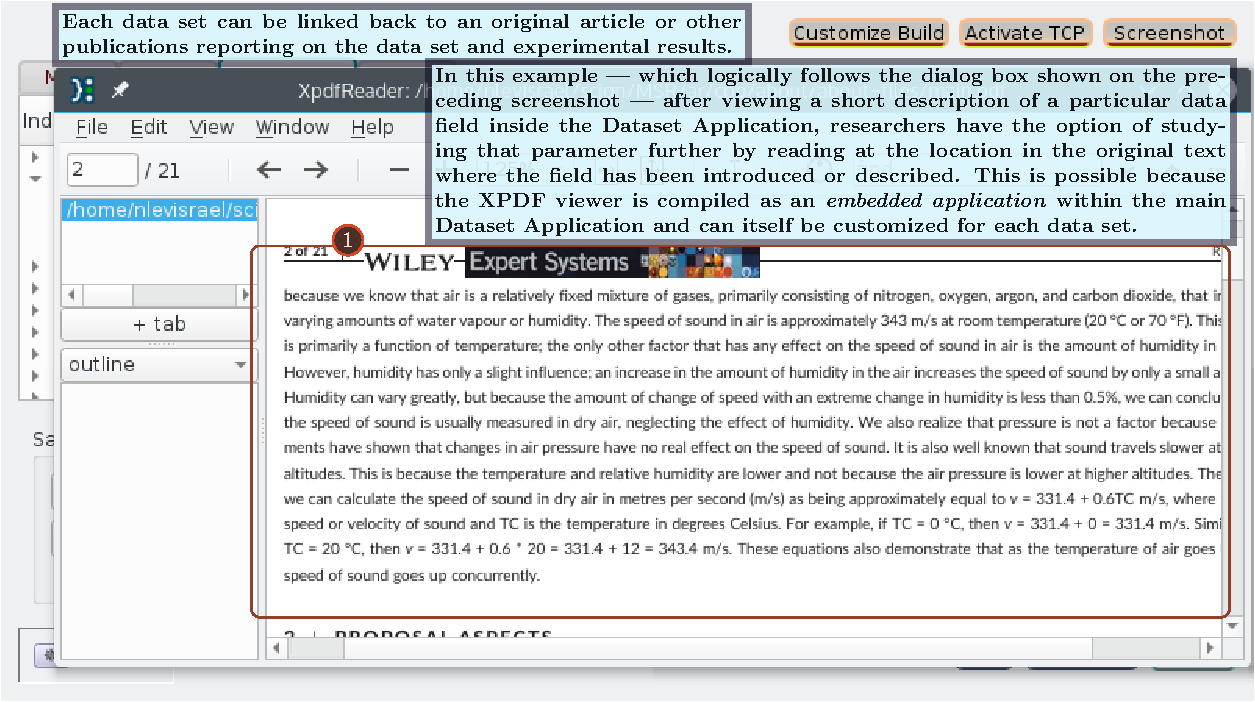
\includepdf[pages=1]{Group_1-8-EmbeddingXPDF.pdf}
%\end{frame}

%\section{Group_1-9-intro}\begin{frame}{\ft{Tree Widget}}
%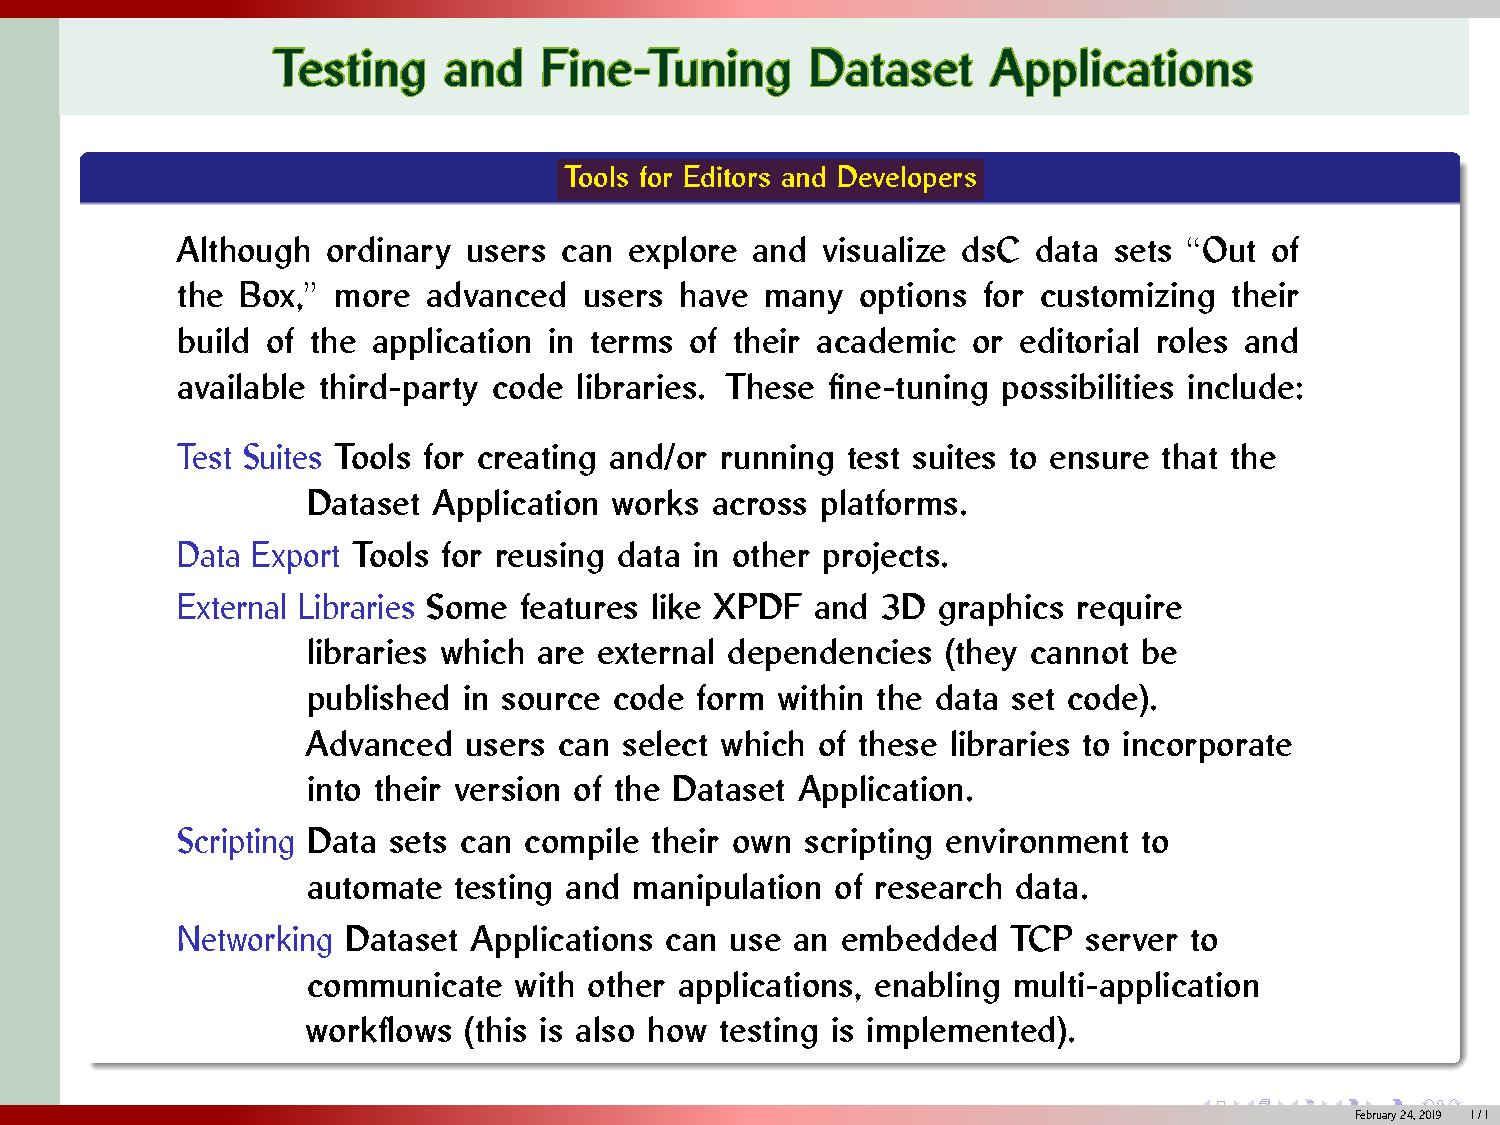
\includepdf[pages=1]{Group_1-9_intro.pdf}
%\end{frame}

%\section{Group_1-9}\begin{frame}{\ft{Tree Widget}}
%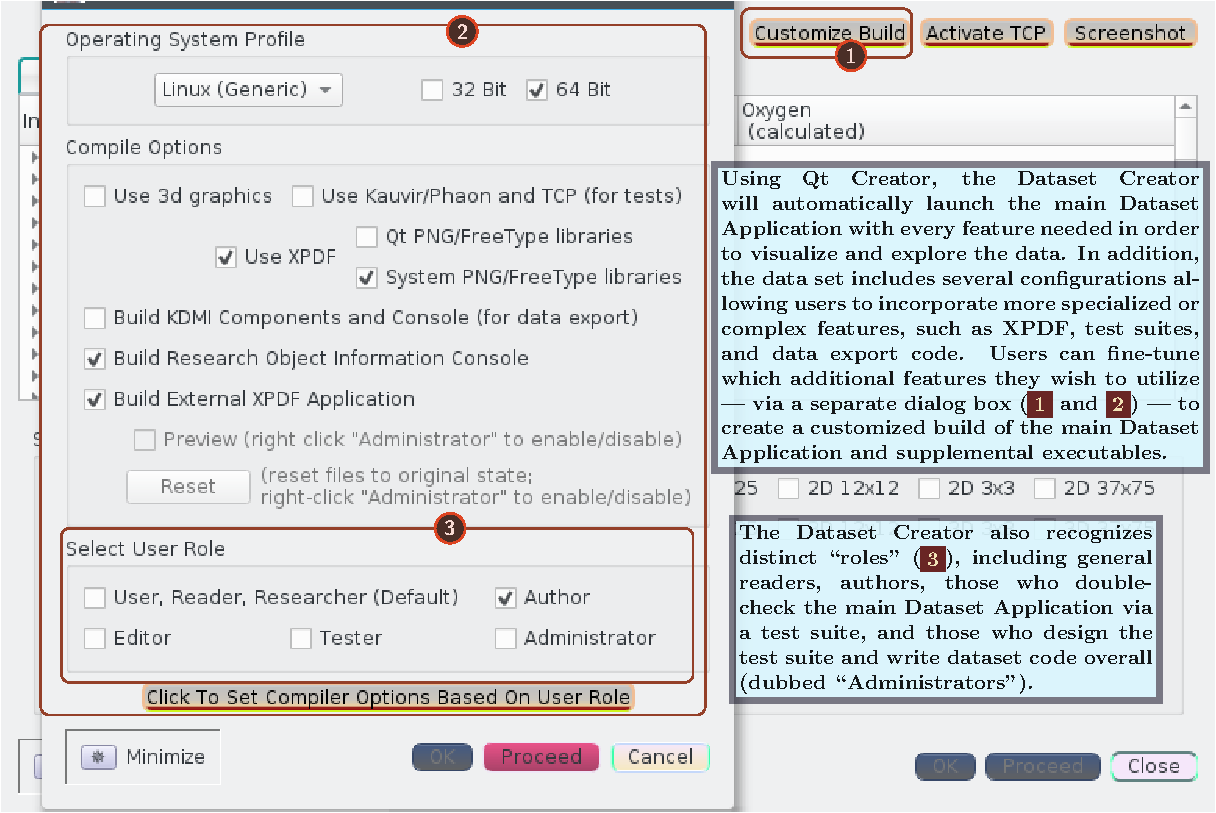
\includepdf[pages=1]{Group_1-9-ConfiguringTheDataSetApplication.pdf}
%\end{frame}

%\section{Group_1-10}\begin{frame}{\ft{Tree Widget}}
%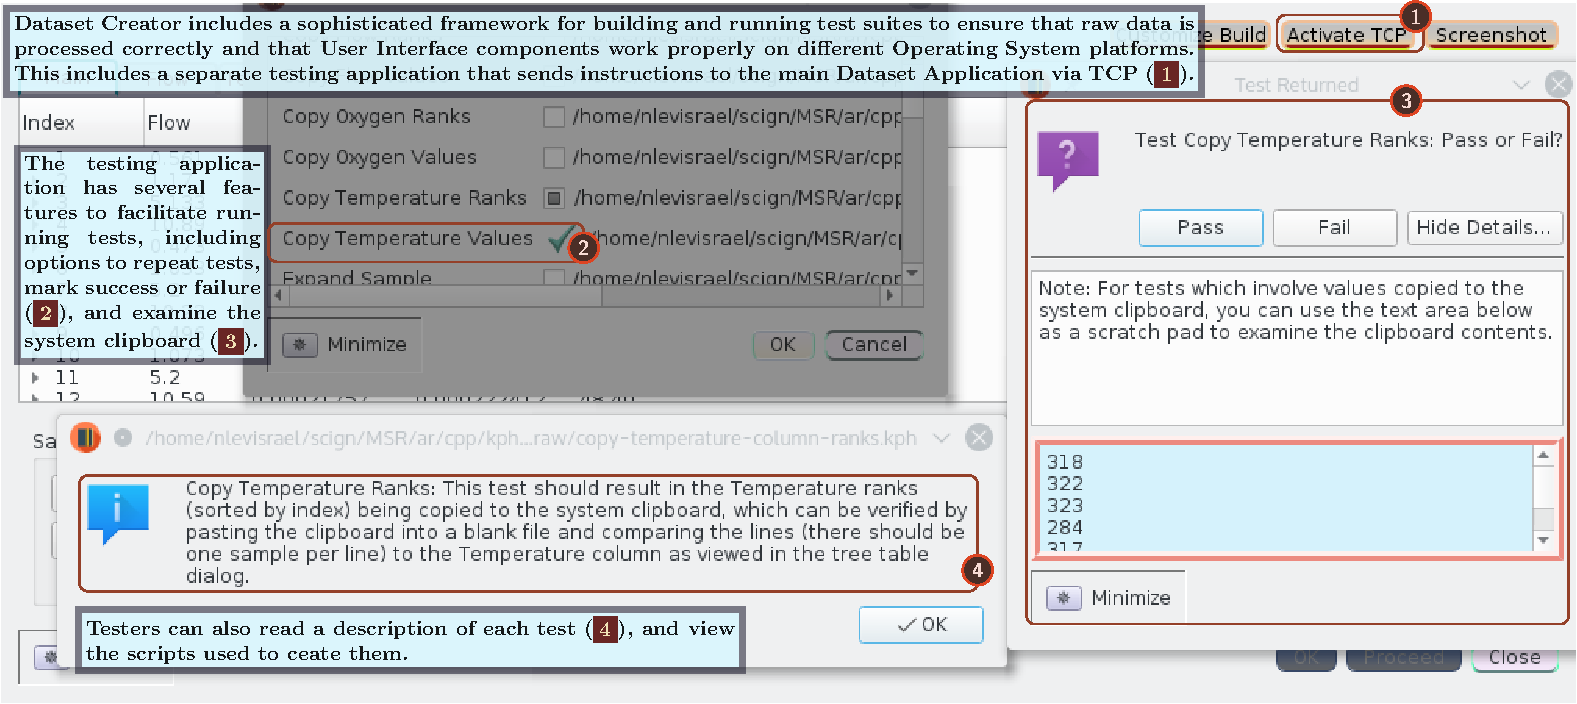
\includepdf[pages=1]{Group_1-10-TestingTheDataSetApplication.pdf}
%\end{frame}

%\section{Group_2-11-intro}\begin{frame}{\ft{Tree Widget}}
%	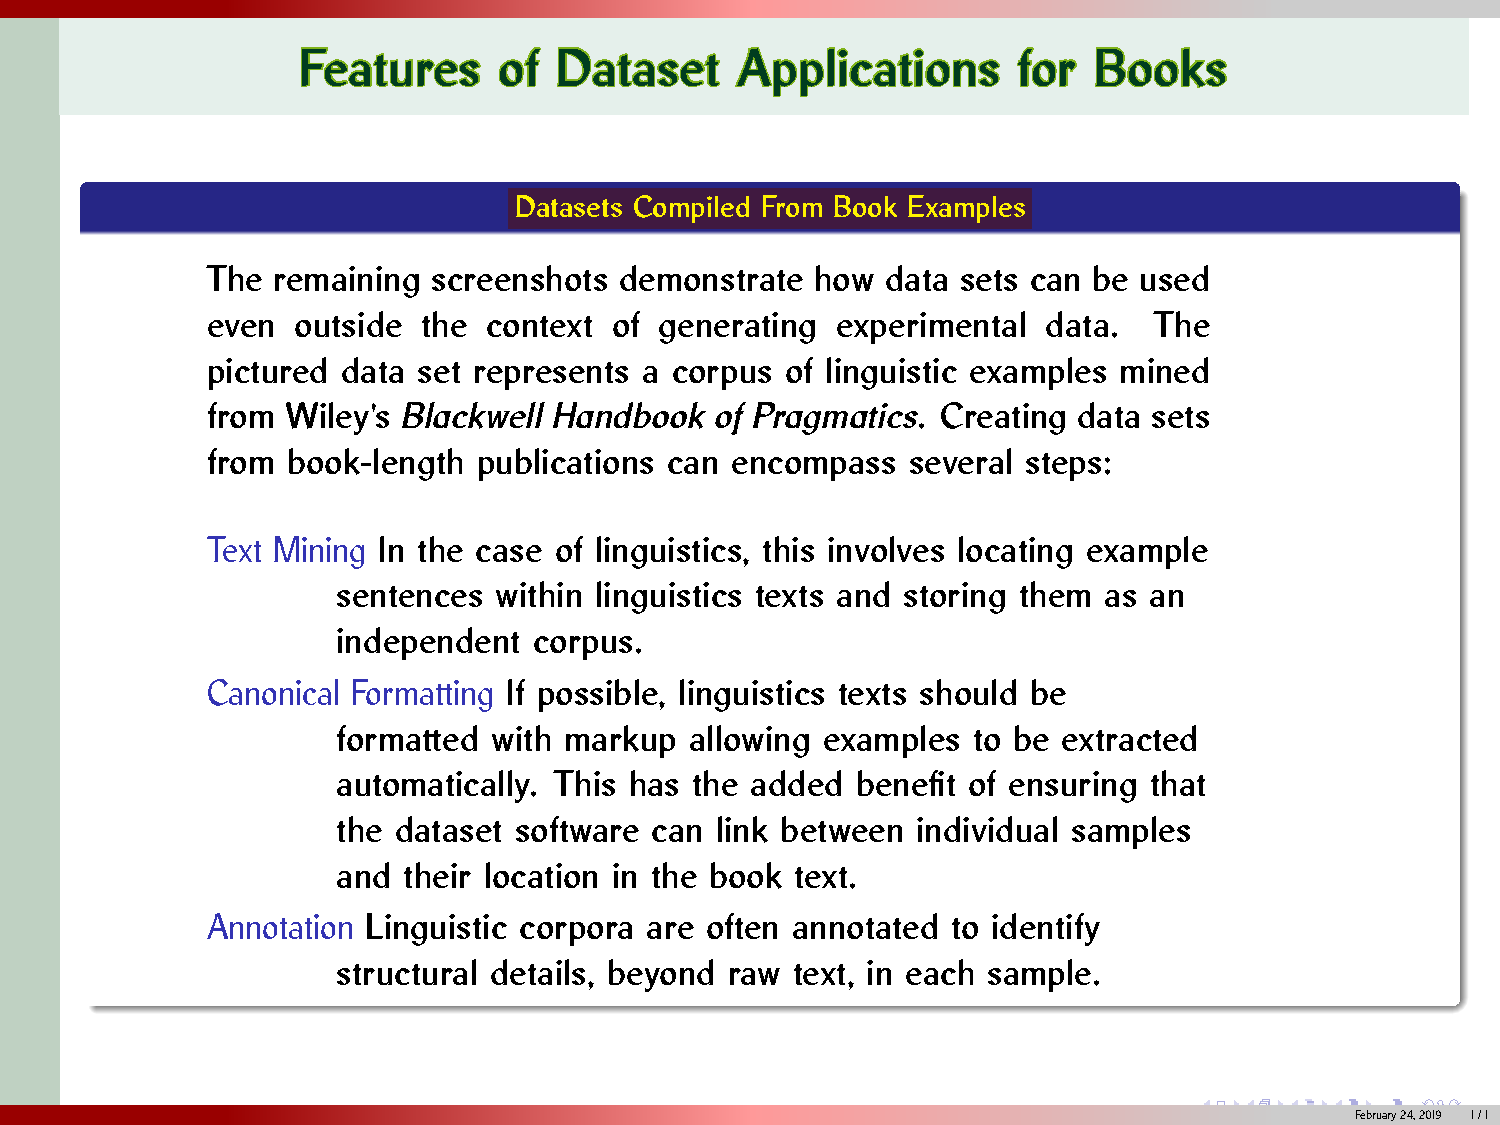
\includepdf[pages=1]{Group_2-11_intro.pdf}
%\end{frame}

%\section{Group_2-11}\begin{frame}{\ft{Tree Widget}}
%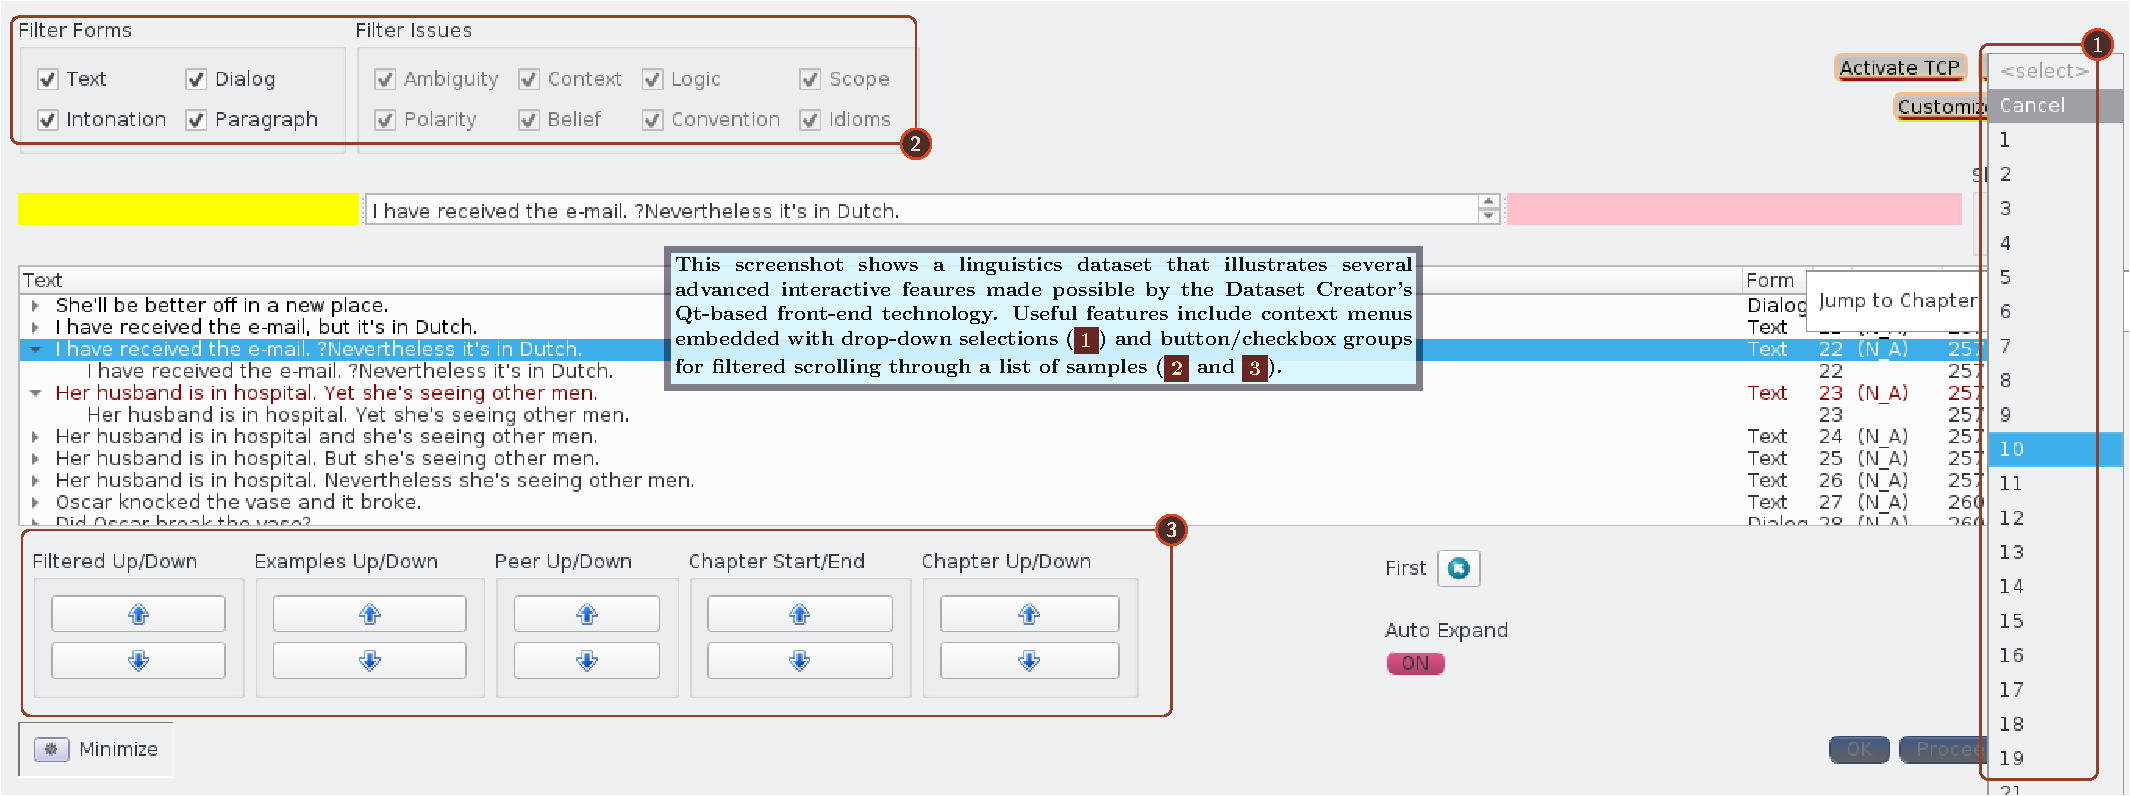
\includepdf[pages=1]{Group_2-11-CreatingADataSetFromABook.pdf}
%\end{frame}

%\section{Group_2-12}\begin{frame}{\ft{Tree Widget}}
%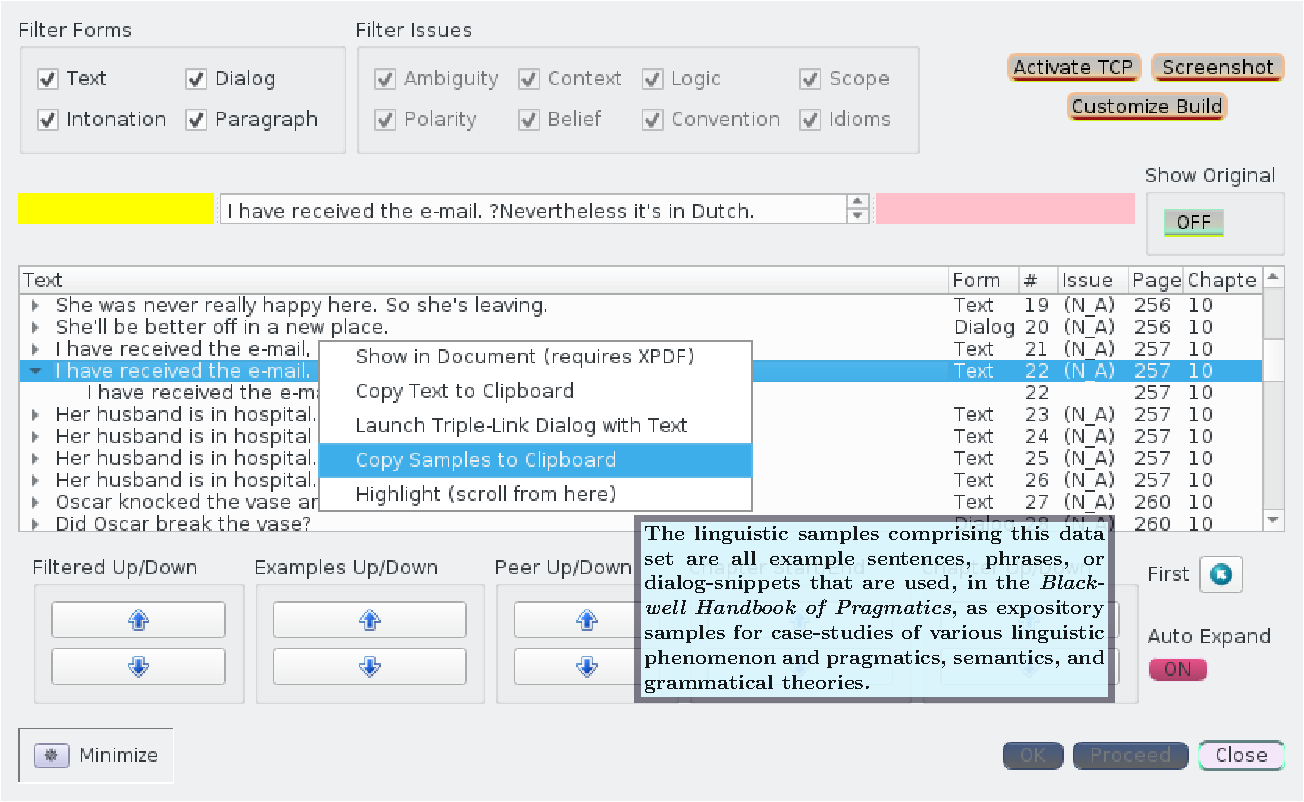
\includepdf[pages=1]{Group_2-12-InteractingWithDataSamples.pdf}
%\end{frame}

%\section{Group_2-13}\begin{frame}{\ft{Tree Widget}}
%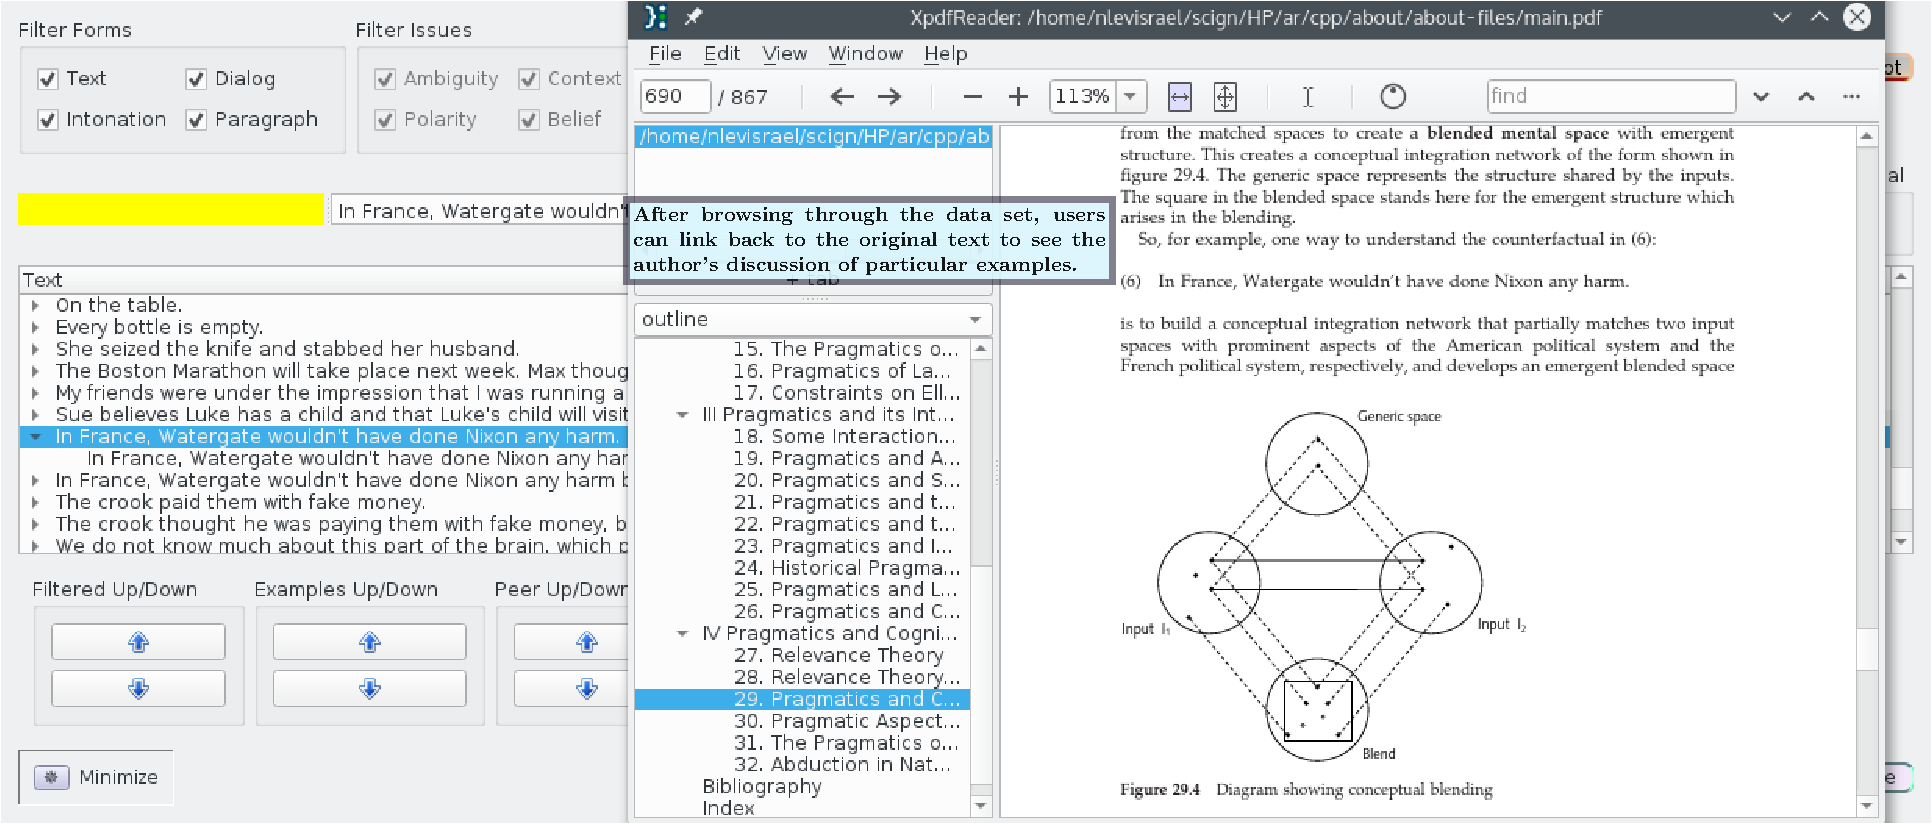
\includepdf[pages=1]{Group_2-13-LinkingBackToTheBook.pdf}
%\end{frame}

%\section{Group_2-14-intro}\begin{frame}{\ft{Tree Widget}}
%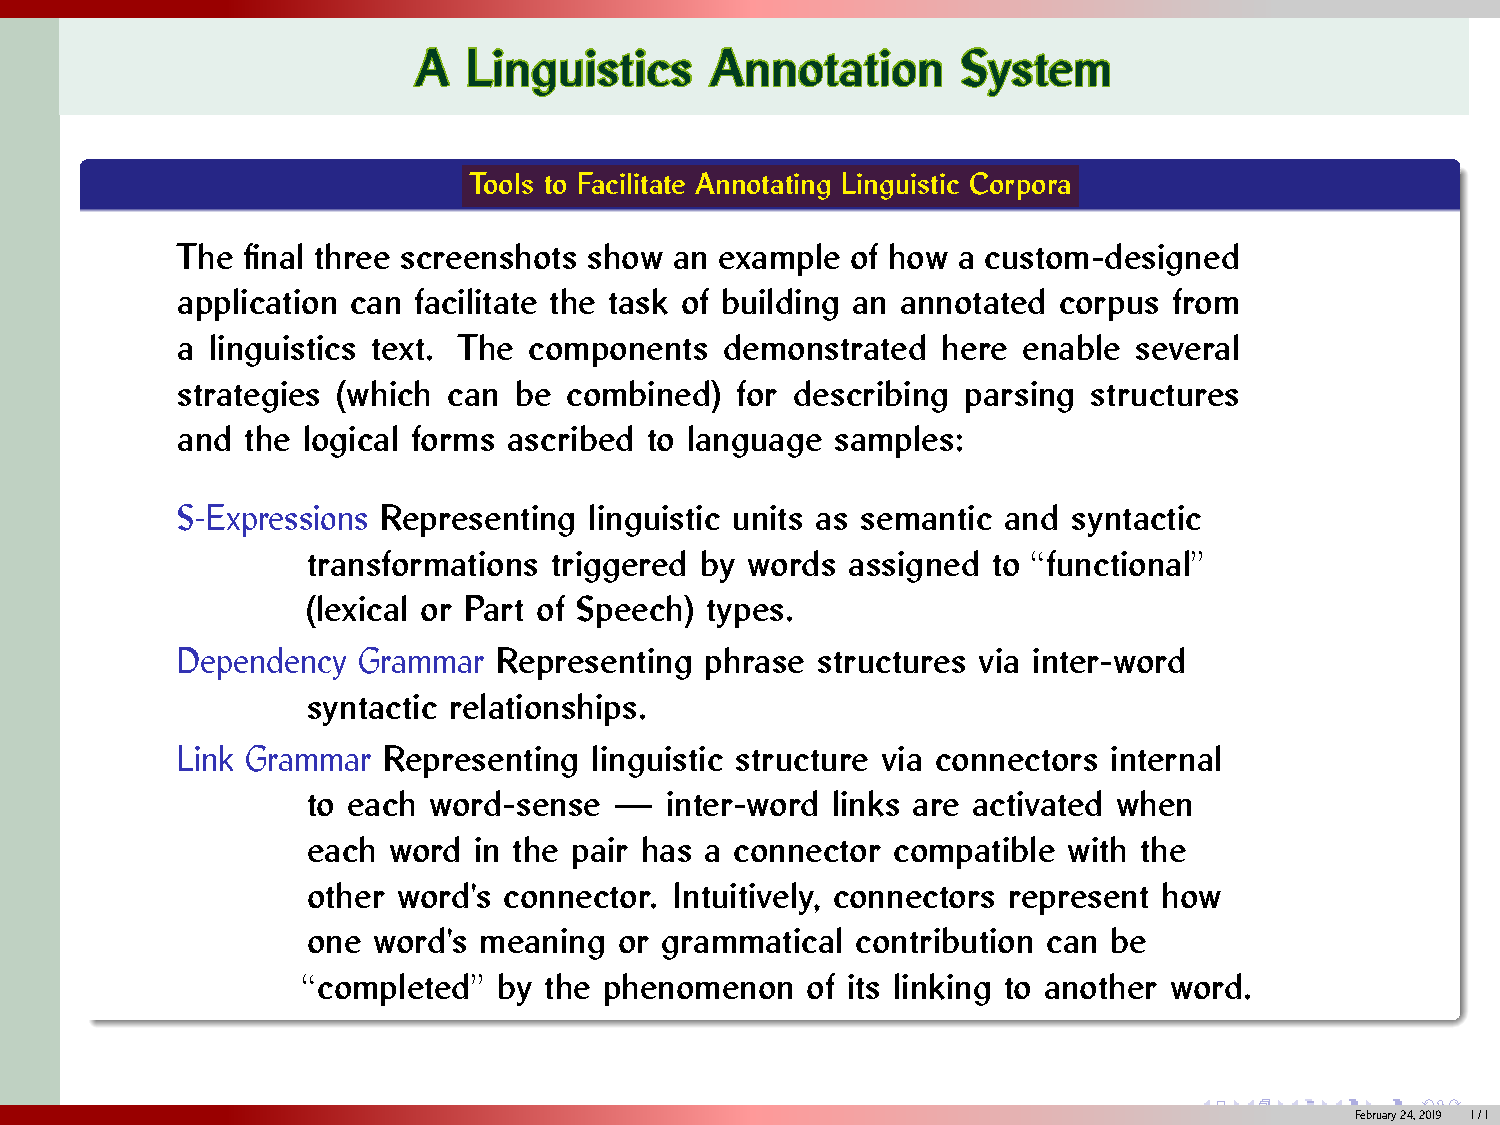
\includepdf[pages=1]{Group_2-14_intro.pdf}
%\end{frame}

%\section{Group_2-14}\begin{frame}{\ft{Tree Widget}}
%	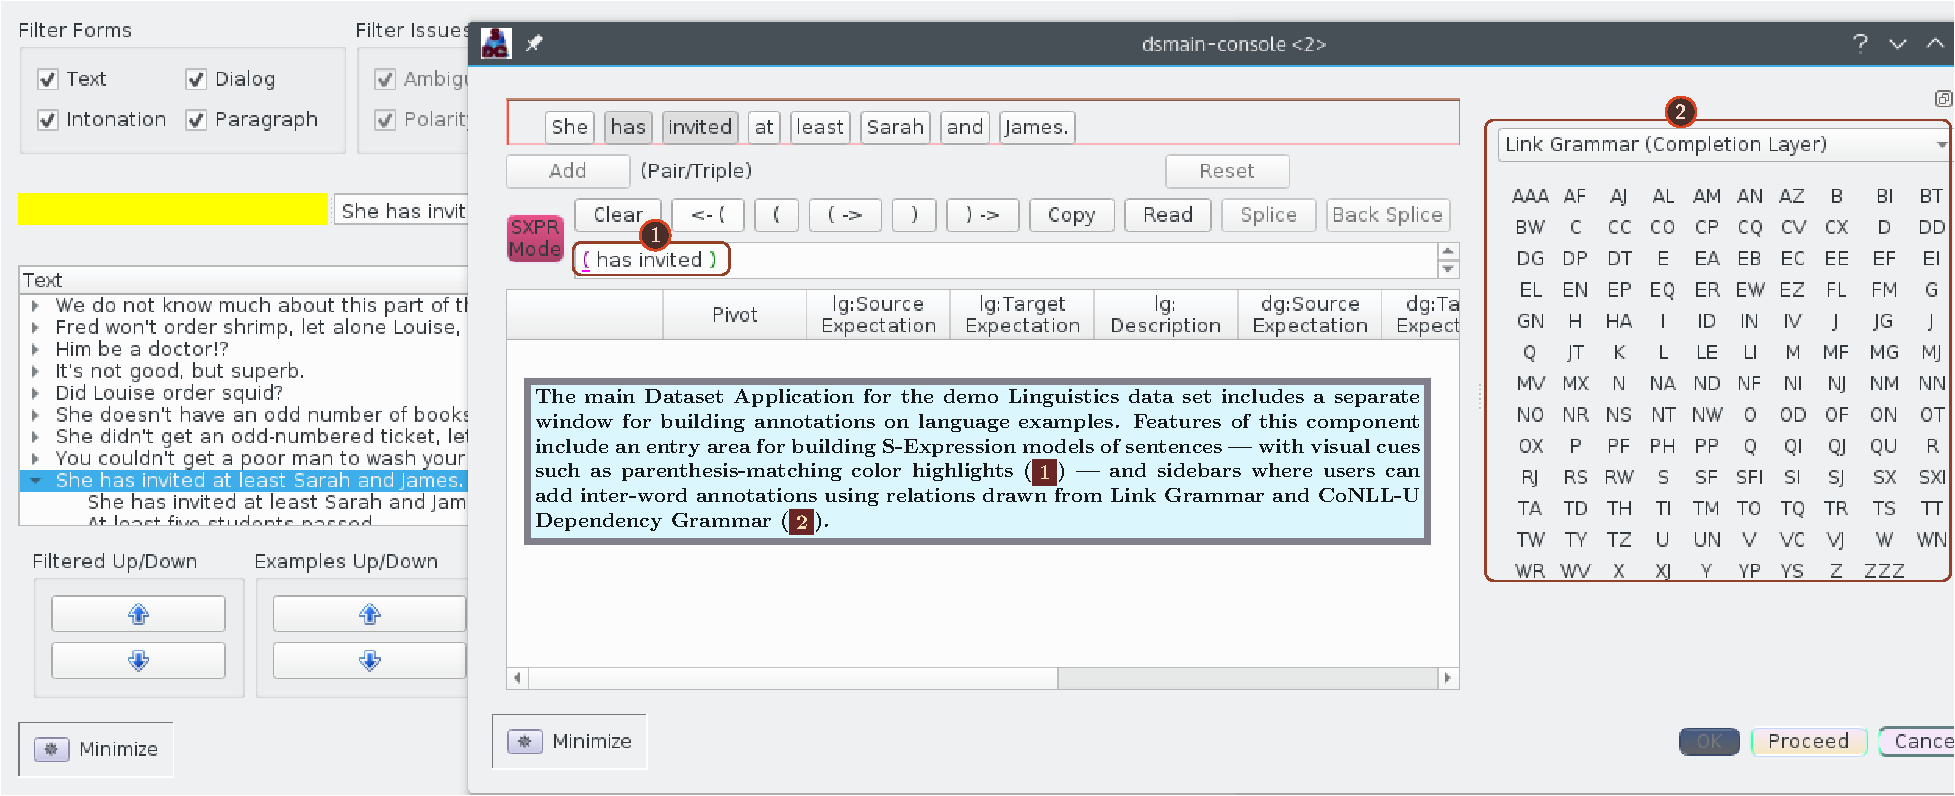
\includepdf[pages=1]{Group_2-14-BuildingParsingModels.pdf}
%\end{frame}

%\section{Group_2-15}\begin{frame}{\ft{Tree Widget}}
%\includepdf[pages=1]{Group_2-15-UsingDockWidgetsForFlexibleLayout.pdf}
%\end{frame}

%\section{Group_2-16}\begin{frame}{\ft{Tree Widget}}
%\includepdf[pages=1]{Group_2-16-LinkAndDependencyGrammarAnnotations.pdf}
%\end{frame}

%}
\part{Publishing}	
\atsp
\begin{frame}{\ft{Technological Components of Dataset Creator}}
\section{Components}

\vspace*{33pt}
{\thrulexrev}
\vspace*{-15pt}

%\MyDiamond{}
{\fontsize{18}{22}\fontfamily{ppl}\selectfont
%\begin{center}
\hspace*{25pt}\begin{minipage}{1.2\textwidth}
\vspace{12pt}


%\definecolor{blback}{RGB}{0,100,100}	
%\definecolor{blfront}{RGB}{0,100,50}

%\fcolorbox{lqboutercolor}{lqbinnercolor}{\begin{minipage}{\textwidth}%
		
%\begin{lightquadblockc}{1,0.4,0.1}{\parbox{24cm}{\hspace*{-9pt}}\vspace{8pt}}
%\begin{minipage}{1.1\textwidth}

{\setlength{\leftmargini}{9pt}\begin{enumerate}
\setlength{\labelsep}{13pt}
\dmitem \textbf{\AtR{} (Application-as-a-Resource)}: \hspace{.25em} 
\AtR{} Applications are self-contained, citable resources and tools which 
can conform to \makebox{modern} resource documentation standards, such as the Research Object protocol.  Dataset Applications can use the \AtR{} tools 
and protocol to create custom desktop-style applications 
for viewing and analyzing research data, while bundling the dataset  and application code into a citable Research Object. 
\vspace{19pt}

\dmitem \textbf{HTXN (Hypergraph Text Encoding Protocol)}:  \hspace{.25em}
HTXN is a protocol for encoding documents' character streams  
and document structure via \q{standoff annotation} (i.e.,  
character encoding is fully separate from structural representation).  
HTXN supports diverse kinds of document models, including 
\LaTeX{}, XML, RDF, and Concurrent/Overlapping XML extensions. 
\vspace{19pt}

\dmitem \textbf{MOSAIC (Multiparadigm Ontologies 
	for Scientific and Academic Publishing)}: \hspace{.25em} 
Mosaic provides data-modeling capabilities which 
reflect a diversity of Information Representation 
paradigms, such as Hypergraphs, Conceptual Spaces, 
and Object-Oriented Simulation.  \\
\vspace{19pt}\hspace{11pt}\raisebox{12pt}{\MySquare}\hspace{11pt}\parbox{19cm}{{\color[rgb]{0.3,0,0.1}{Mosaic includes 
the Mosaic/HTXN Semantic Document Infoset (MH-SDI) and 
Mosaic Plugin Framework (MPF) (see slides 19-26).}}}
\vspace{19pt}  

\end{enumerate}
}

%\end{minipage}
%\end{lightquadblockc}
\end{minipage}
}

%}
%\end{minipage}
%\end{center}
%}

\end{frame}



\begin{frame}{\ft{A3R Document Viewers}}
\section{Publishing Slide 1}
\doubleFrame{A3R applications may embed viewers for 
%popular 
document formats such as e-Pub, HTML, and PDF; 
 %The application may 
then supplement conventional publications 
with special components 
%software %components, perhaps 
customized for 
individual manuscripts --- here, a widget 
allowing readers to visually explore patterns in 
classical Indian music.}

\begin{tikzpicture}
\nodeincludegraphicsTRRS{0.95}{2cm}{3cm}{5cm}{.5cm}{pics/Pub-2.png}

% \node [anchor=west,fill=brown!20!white,inner sep=7, text width=14cm]
%  (longnote) at (5.5,7) {%  %{\color{rb!85!red}{
%  {\cframedbox{\large \textbf{EC1}}}};

\end{tikzpicture}


\end{frame}


\atsp
\begin{frame}{\ft{\AtR{} Document Viewers as Embedded Components}}
\section{Publishing Slide 2}
\doubleFrameY{\textwidth}{-7.5pt}{1.006\textwidth}{0.96\textwidth}{1pt}{%
Document Viewers may also be embedded in 
host applications which provide domain-specific 
\makebox{visualization} capabilities.  For example, chemistry papers 
might be viewed within IQmol (a Qt-based program for molecular visualization and physical/chemical analysis) via an \AtR{} document-viewer plugin.}

\begin{tikzpicture}
\nodeincludegraphicsTRRS{.8}{2cm}{2.7cm}{2cm}{0}{pics/Pub-1.png}

% \node [anchor=west,fill=brown!20!white,inner sep=7, text width=14cm]
%  (longnote) at (5.5,7) {%  %{\color{rb!85!red}{
%  {\cframedbox{\large \textbf{EC2}}}};

\end{tikzpicture}


\end{frame}




\begin{frame}{\ft{Document Viewers Augmented With APIs}}
\section{Publishing Slide 3}
\doubleFrame{Another strategy for interactive publications is linking documents with APIs maintained by publishers, or 
by cultural or educational institutions.}

\begin{tikzpicture}
\nodeincludegraphicsTR{2.7cm}{2cm}{pics/Pub-3.png}

 \node [anchor=west,bottom color=yellow!20!orange, top color=darkRed!70!red,inner sep=3, text width=14cm]
  (longnote) at (2.9,10.3) {\vspace{-7pt}%  %{\color{rb!85!red}{
  {\cframedbox{\Large \textbf{As an example, documents 
mentioning artifacts held in a \makebox{museum} can provide features to 
view more information about those museum-pieces through the host 
institution's API. 
}}}};

\end{tikzpicture}


\end{frame}




\begin{frame}{\ft{EC-4}}

\doubleFrame{EC4.}

\begin{tikzpicture}
\nodeincludegraphicsTR{2.7cm}{2cm}{pics/Pub-4.png}

 \node [anchor=west,fill=brown!20!white,inner sep=7, text width=14cm]
  (longnote) at (5.5,7) {%  %{\color{rb!85!red}{
  {\cframedbox{\large \textbf{EC4}}}};

\end{tikzpicture}


\end{frame}




\begin{frame}{\ft{How NCN Addresses Limitations of 
				the Semantic Web}}
\section{Semantic Web}
\vspace{.5em}	

\definecolor{blueback}{RGB}{0,100,100}	
\definecolor{bluefront}{RGB}{0,100,50}
\definecolor{htxt}{rgb}{0.2,0.15,0.1}

{\hspace*{-2pt}
\begin{minipage}[c]{\textwidth}\Large\centering
		\color{htxt} 	
\vspace{.1em}\textbf{%	
Many experts have critiqued the Semantic Web for 
lacking conceptual rigor, adequate modeling for 
multi-scale information, and 
intrinsic representations for Quality 
Assurance Requirements.
To address these limitations, NCN 
introduces new Semantic Web technologies 
with the following features:}\end{minipage}}
\vspace{1.4em}
	
{\Large\fontfamily{uhv}\selectfont
\begin{minipage}{\textwidth}
\fcolorbox{fcBoxColor}{blueback}{
\begin{minipage}{.99\textwidth}
\vspace*{12pt}	
\hspace{3pt}%
\fcolorbox{fcBoxColor}{white}{\begin{minipage}{.97\textwidth}%
\vspace{.8em}
{\centerline{\LARGE\color{darkRed!50!red} \textbf{The 
			Application-as-a-Resource (\AtR{}) Model}}}
\vspace{1em}
{\setlength{\leftmargini}{25pt}
{\Large\begin{itemize}
\sqitem {\lsep} \parbox[t]{19.5cm}{\AtR{} Applications are self-contained, citable resources and tools which 
can conform to \makebox{modern} resource documentation standards, such as the 
Research Object protocol.}
\vspace{.8em}
\sqitem {\lsep} \parbox[t]{18.8cm}{\AtR{} includes a 
representation for natural language publications 
(e.g., books and articles) that unifies different 
manuscript formats (such as XML, \LaTeX{}, 
and XCONCUR).}
\end{itemize}}}\vspace{12pt}
\end{minipage}}\\\\\\
\vspace*{1em}
\hspace{-1pt}\fcolorbox{bluefront!25!fcBoxColor}{white}{\begin{minipage}{.97\textwidth}%
\vspace{.8em}
{\centerline{\LARGE\color{darkRed!50!red} \textbf{Multiscale, Requirements-Focused Resource Description}}\vspace{.8em}}
{\setlength{\leftmargini}{25pt}
{\Large%\begin{minipage}{.96\textwidth}
\begin{itemize}
\sqitem {\lsep} \parbox[t]{19cm}{NCN/\AtR{} 
(combinatorially called \q{NA3}) incorporates 
Semantic Web alternatives with greater Quality 
Assurance precision, such as Conceptual Space 
Markup Language.}
\vspace{.5em}  
\sqitem {\lsep} Hypergraph-based Resource Framework 
to intrinsically support multi-scale data structures.
\vspace{.5em}   
\sqitem {\lsep} \parbox[t]{18.5cm}{
Workflow-oriented \q{Meta-Procedure} Interface Definition 
framework to enforce \\procedural alignment among applications.
}
 \vspace{1.5em}
\end{itemize}%\end{minipage}
}
}
\end{minipage}}\end{minipage}}
\end{minipage}}
\end{frame}


\part{Thanks}
\atsp
\begin{frame}{\ft{Thank You!}}
	\section{Thanks}
{\LARGE
\vspace{.25em}
\hspace{2.9em}\colorbox{pink!40!black}	
{\parbox{19cm}{\vspace{6pt}\raisebox{6pt}{%
 \hspace{4pt}\colorbox{white}{\setlength{\fboxsep}{1.65em}
   \hspace{-4pt}\raisebox{3.8em}{
   {\color{pink!35!black}{\parbox{18cm}{\vspace{7pt}\framebox{\begin{minipage}{.7\textwidth}\centering
	  {\color{blGreen!40!blbl}\textbf{Please contact 
	  Linguistic Technology Systems for 
	  more information  
	  about Dataset Creator:\\ 
      (917) 817-2184\\amy.neustein@verizon.net}}
	 \end{minipage}}}}}}\hspace{8pt}}\hspace{5pt}}}}}
	 
\vspace{22pt}

\hspace*{25pt}\begin{minipage}{24cm}
%\begin{adjustwidth*}{-1em}{} 
\begin{tikzpicture}


%\nodeincludegraphicsLOCTRV{11.1,5.9}{0.4}{0cm}{2cm}{6cm}{2cm}{lp/lp3.png}

\nodeincludegraphicsLOCTRV{0,0}{0.5}{0cm}{5.7cm}{0cm}{1cm}{lp/lp6.png}
\nodeincludegraphicsLOCTRV{14,1.6}{0.7}{12cm}{3cm}{0cm}{2cm}{lp/lp2.png}
\nodeincludegraphicsLOCTRV{20,0.2}{0.37}{0cm}{5.7cm}{0cm}{1cm}{lp/lp4.png}
\nodeincludegraphicsLOCTRV{22,5.2}{0.5}{4cm}{2cm}{13cm}{4cm}{lp/lp7.jpg}

%\nodeincludegraphicsLOCTRV{0.5,1.2}{0.4}{1cm}{5cm}{6cm}{2cm}{lp/lp5.png}

%\nodeincludegraphicsLOCTRV{3.1,3.2}{0.3}{4.5cm}{1cm}{0.5cm}{0.5cm}{lp/lp2.jpeg}


%\nodeincludegraphicsLOCTRV{6.2,3.7}{0.24}{0cm}{2cm}{2cm}{0cm}{flowers.jpg}
%\nodeincludegraphicsLOCTRV{0.6,0.7}{0.2}{0cm}{4cm}{0cm}{0cm}{iqMOL-5.png}

\end{tikzpicture}
%\end{adjustwidth*}
\end{minipage}	 
\end{frame}



\end{document}
